\documentclass[a4paper,11pt]{report}
\makeatletter
\renewcommand*\@makechapterhead[1]{%
  \vspace*{50\p@}%
  {\parindent \z@ \raggedright \normalfont
    \ifnum \c@secnumdepth >\m@ne
  %      \huge\bfseries \@chapapp\space \thechapter
  %      \par\nobreak
 %       \vskip 20\p@
    \fi
    \interlinepenalty\@M
    \Huge \bfseries \thechapter \space #1\par\nobreak
    \vskip 10\p@
  }}
\renewcommand*\@makeschapterhead[1]{%
  \vspace*{50\p@}%
  {\parindent \z@ \raggedright
    \normalfont
    \interlinepenalty\@M
    \Huge \bfseries  #1\par\nobreak
    \vskip 40\p@
  }}
\makeatother

\setlength{\parindent}{0cm}

\usepackage[nottoc]{tocbibind}
\usepackage[labelfont=bf]{caption}
\usepackage{epsfig}
%\usepackage{times}
\usepackage{multirow}
\usepackage{float}
\usepackage{subcaption}
\usepackage{longtable}
\usepackage[nomessages]{fp}
\usepackage{tabularx}
\usepackage{comment}
\usepackage{KTHEEtitlepage}
\usepackage[hmargin=2.5cm,vmargin=2.5cm]{geometry}
\usepackage{fancyhdr}			% contains customizeable headers and footers
\pagestyle{fancy}
\usepackage{wrapfig}
\usepackage{booktabs}
\usepackage{graphicx}
\usepackage{fancyref}
\usepackage{amsmath,amssymb}   % Contains mathematical symbols
%\usepackage[english]{babel}
\usepackage[T1]{fontenc}
\usepackage{pslatex}
\usepackage[utf8]{inputenc}
\usepackage{natbib}  %Nice author (year) citations
%\usepackage[round,authoryear]{natbib}  %Nice author (year) citations

%\addtolength{\textheight}{-8mm}% Adds it to the text height
%\headheight = 12mm


%\addtolength{\topmargin}{-30mm}% Removes 30mm from the top margin
%\addtolength{\textheight}{30mm}% Adds it to the text height

\usepackage{hyperref}
\hypersetup{
    colorlinks=true,       % false: boxed links; true: colored links
    linkcolor=black,          % color of internal links (change box color with linkbordercolor)
    citecolor=black,        % color of links to bibliography
    filecolor=black,      % color of file links
    urlcolor=blue           % color of external links
}
\usepackage{array}
\usepackage[final]{pdfpages}
\usepackage{nomencl}
\usepackage[num,english]{isodate}
\usepackage{acronym}
\makenomenclature
\renewcommand{\nomname}{List of Acronyms}
\newcommand*{\nom}[2]{#1\nomenclature{#1}{#2}}





















\newcommand{\newPar}{\\[11pt]}


\newcommand{\surname}{Diaz}
\newcommand{\firstname}{Rene}
\newcommand{\mail}{radm@kth.se}
\newcommand{\schoolDepartment}{Department of Machine Design}
\newcommand{\schoolName}{Royal Institute of Technology}
\newcommand{\schoolAcronym}{KTH}
\newcommand{\reportTitle}{A library on the Robot Operating System (ROS) for Model Predictive Control implementation}
\newcommand{\reportSubtitle}{}
\newcommand{\reportDate}{December 2014}
\newcommand{\reportRefNr}{}

\begin{document}
\pagenumbering{roman} %Use roman numbering for preface
\ititle{\reportTitle}
\isubtitle{\reportSubtitle} % Optional
\idate{\reportDate}
\irefnr{\reportRefNr}
\iauthor{\firstname \hspace{0pt} \surname}
\makeititle

\pagebreak
\begin{abstract}
\end{abstract}

\pagebreak
{\listoffigures}
{\tableofcontents}
\pagebreak

\cleardoublepage
\pagenumbering{arabic}

\pagestyle{fancy}
\fancypagestyle{plain}{%
\fancyhf{} % clear all header and footer fields
\fancyhead[L]{\slshape \leftmark}
\fancyhead[C]{}
\fancyhead[R]{\slshape \rightmark}
\fancyfoot[C]{\thepage}
\renewcommand{\headrulewidth}{0.4pt}
\renewcommand{\footrulewidth}{0pt}}
\headheight = 14pt

\printnomenclature[50pt]
\chapter{Introduction}
\label{chap:Introduction}
%\section{Background}
\label{chap:Background}

The Mechatronics Research group at Simon Bolivar University in Caracas, Venezuela is focused on the development of solutions based on the integration of knowledge in the fields of Automatic Control, Computer Science, AI and Robotics, Electronics and Mechanics. This development is made on a project based strategy, with projects coming from both industry and academia. One of the projects that has been developed during the last years is the submarine of the university, named PoseiBot. The development of this submarine robotic platform has been made in several phases through the years. In the latest phase, a Model Predictive Control (MPC) strategy was implemented to control the submarine achieving good results in terms of the control effort, error reduction and robustness. MPC is an advanced control technique based on solving an optimal control problem with a finite prediction horizon in each sample. MPC is commonly applied to large systems with slow dynamics, but recently with the increase of computational power and the development of new algorithms that are more efficient, systems with faster dynamics are being targeted to be controlled by predictive methods. This was implemented through communication of the submarine's microcontroller to a remote computer out of the water using serial wired communication to a flotation device that communicates wirelessly with the remote computer. In the computer, signal acquisition  and data processing was done via LabVIEW \texttrademark  and MATLAB\textsuperscript{\textregistered}, respectively. \\

Another project developed in the group is the usage of quadrotors as a robotic platform for powerline inspection, where DETAILS ABOUT THE CONTROL STRATEGIES AND HOW IT IS IMPLEMENTED. Due to the wind conditions around the powerlines to be inspected, a robust control algorithm is required to assure a safe operation of the quadrotor while maneuvering around the lines.\\

Based on the requirements set by the aforementioned projects, there has been an increasing interest in advanced control techniques and specially MPC applications for both platforms. MPC has been proven as an efficient tool for solving multivariable control problems that might be difficult to decouple, in plants that might have some restrictions in some variables and might even be nonlinear. MPC can handle all of these requirements satisfactorily while being optimal in the solution, which is important in cases where resources are limited.\\




But in order to provide a solution that could fit both applications in a relatively quick way, some standardization and abstraction is required in the solution. That is where the benefits of using ROS apply, and it also represented an opportunity to extend the usage of this tool within the group. FIX MEEE

%\section{Bibliographic Revision}
\label{chap:Bibliographic_Revision}




%\section{Purpose}
\label{chap:Purpose}

The purpose of this project is the creation of a ROS package to implement MPC strategies in different platforms in a standard and abstract way. The standard characteristic is necessary to get a package that is easy to use without needing to know how it works internally. The abstraction required comes from the fact that the software must work equally good independently of the platform that is being controlled. Of course, there are limitations on how much abstraction can be obtained, since every application will require the development of a process model for the package to use. However, the goal is to use the properties of ROS to achieve this.\\

To reach this goal, the first activity to do will be an extensive bibliographic revision about MPC and its varieties, either theoretically and implemented in different systems. Another topic included in this revision is quadratic programming, since the interest is to apply MPC with constraints. When the MPC problem is not constrained the control law can be calculated exactly, but when constraints are added the solution must be obtained numerically, and there is when quadratic programs arise. \\

After this phase, the focus will be the design of the organization and development of the package. This is an important phase of the project because a proper design will allow a modular organization of the functionality, i.e. the nodes in the package will be enabled to be used in different combinations without altering the way the software works. The development is carried out in an iterative way, so the code can be tested and improved in each iteration. \\

The third phase consists in the creation of a demonstrative platform to use it as an overall test for the package. This includes the creation of a Model and Simulator classes for such system. The model used is kept simple to ease the validation of the results. The chosen system for this purpose is a water recirculation system with two tanks, that is used in the Automatic Control courses. This will save the modeling work, since this is a well known plant. \\

At this point, the MPC package will be already running properly, and then the time to try it in a relevant platform comes. The modeling of the quadrotor platform will be performed to use it with the MPC package and perform simulated tests in trajectories of interest. This phase may require several tests in order to characterize and obtain the properties of the quadrotor if there is no relevant work available about it. The model also requires a validation process for itself to prove that it works in an adequate manner. 

%\section{Delimitations}
\label{chap:Delimitations}


\section{Background}

The Mechatronics Research group at Simon Bolivar University in Caracas, Venezuela is focused on the development of solutions based on the integration of knowledge in the fields of Automatic Control, Computer Science, AI and Robotics, Electronics and Mechanics. This development is made on a project based strategy, with projects coming from both industry and academia. One of the projects is focused on the development of underwater inspection using the underwater robot developed in the group called PoseiBot. The development of this underwater robotic platform has been made in several phases through the years. In the latest phase, a Model Predictive Control (MPC) strategy was implemented by Molero et al. \cite{Molero2011} to control the submarine in order to achieve accuracy control in PoseiBot in terms of the control effort, error reduction and robustness. MPC is an advanced control technique based on solving an optimal control problem with a finite prediction horizon in each iteration. MPC is commonly applied to large systems with slow dynamics, but recently with the increase of computational power and the development of new algorithms that are more efficient, systems with faster dynamics are being targeted to be controlled by predictive methods. This was implemented through communication of PoseiBot's microcontroller to a remote computer out of the water using serial wired communication to a flotation device that communicates wirelessly with the remote computer. In the computer, signal acquisition  and data processing was done via LabVIEW \texttrademark  and MATLAB\textsuperscript{\textregistered}, respectively. \\

Another project developed in the group is the usage of helicopter models as a robotic platform for powerline inspection. Due to the wind conditions around the powerlines to be inspected, a robust control algorithm is required to assure a safe operation of the quadrotor while maneuvering around the lines. There is a strong interest on using instead the quadrotor available in the research group instead of the helicopter because of the increased stability. \\

Based on the requirements set by the aforementioned projects, there has been an increasing interest in advanced control techniques and specially MPC applications for both platforms. MPC has been proven as an efficient tool for solving multivariable control problems that might be difficult to decouple in plants that might have restrictions in the variables and might even be nonlinear. MPC can handle all of these requirements satisfactorily while being optimal in the solution, which is important in cases where resources are limited.\\




But in order to provide a solution that could fit both applications in a relatively quick way, some standardization and abstraction is required in the solution. That is where the benefits of using ROS apply, and it also represented an opportunity to extend the usage of this tool within the group.


\section{Purpose}

The purpose of this project is the creation of a ROS package to implement in a standard and abstract way MPC strategies in different platforms . The standard characteristic is necessary to get a package that is easy to use without needing to know how it works internally. The abstraction required comes from the fact that the software must work equally good independently of the platform that is being controlled. Of course, there are limitations on how much abstraction can be obtained, since every application will require the development of a process model for the package to use. However, the goal is to use the properties of ROS to achieve this.\\

To reach this goal, the first activity to do will be an extensive bibliographic revision about MPC and its varieties, either theoretically and implemented in different systems. Another topic included in this revision is quadratic programming, since the interest is to apply MPC with constraints. When the MPC problem is not constrained the control law can be calculated exactly, but when constraints are added the solution must be obtained numerically, and there is when quadratic programs arise. This happens for linear systems and/or linearized systems, which are the object of interest in this phase of the project.\\

After this phase, the focus will be the design of the organization and development of the package. This is an important phase of the project because a proper design will allow a modular organization of the functionality, i.e. the nodes in the package will be enabled to be used in different combinations without altering the way the software works. The development is carried out in an iterative way, so the code can be tested and improved in each iteration. \\

The third phase consists in the creation of a demonstrative platform to use it as an overall test for the package. This includes the creation of a Model and Simulator classes for such system. The model used is kept simple to ease the validation of the results. The chosen system for this purpose is a water recirculation system with two tanks, that is used in the Automatic Control courses. This will save the modeling work, since this is a well-known plant. \\

At this point, the MPC package will be already running properly, and then the time to try it in a relevant platform comes. The modeling of the quadrotor platform will be performed to use it with the MPC package and perform simulated tests in trajectories of interest. This phase may require several tests in order to characterize and obtain the properties of the quadrotor if there is no relevant work available about it. The model also requires a validation process for itself to prove that it works in an adequate manner. 

\section{Bibliographic Revision}

Even though MPC has been proven since long time ago to be applicable for different types of plants and processes, it took some time until the industry embraced it as the powerful tool it is. One of the first attemps to show the pros and cons of MPC is described  by Richalet in \cite{Richalet1993}. In this paper, the benefits of implementing MPC are addressed from an industrial point of view, as well as the differences in the approach required to apply it in a proper way. The diversity of applications for MPC is also a topic in this paper: two cases are conducted, one with slow dynamics systems and one in a system with quick dynamics; being able to handle both satisfactorily. An important conclusion from this paper is that the difference in application compared to traditional control techniques is that the effort is centered on the development of the model, not in the tuning of the controller. If a proper model is developed, the tuning of the controller consists on a proper choice of the horizons and weight matrices. On the other side, this requires a higher level of training for the staff in charge of the system.\\

In order to take advantage of this new engineering approach for the application of this technique, there have been several attempts to provide a platform to ease the control and focus on the modeling work. Most implementations in research are implemented using MATLAB\textsuperscript{\textregistered} as in \cite{Gabrielsson2012}, \cite{Molero2011}, \cite{Kristoffersson2006} and \cite{Johansson2012} to mention some examples.\\

In \cite{Gabrielsson2012}, a linear MPC strategy is used to provide a system of water dams an adequate flow of water required for the paper mills while maintaining the water levels among some defined boundaries and optimizing the use of it. In this thesis report it is easy to see practically the point that was made before: a good part of the work is done in the development of a suitable model, afterwards the tuning of the MPC strategy is reduced to the tuning of the weight matrices, the prediction and control horizons and the size of the control time step. The MPC technique in this report is performed in MATLAB \textsuperscript{\textregistered}, using a quadratic cost function and state estimation via Kalman. In this case, the system dynamics are not so fast, so the computational power provided by MATLAB \textsuperscript{\textregistered} is enough to solve the problem within the sampling time restrictions.\\

In \cite{Molero2011}, the problem to solve is the trajectory tracking of a underwater ROV. In this case, the MPC formulation used is a particular one because the constraints in the control and state variables are translated to the cost function directly using penalty functions. In this way, each constraint has a penalty cost associated that goes into the objective function. The implementation used a combination of wired and wireless technology for the data sending/receiving process, which was sent to a remote computer performing the MPC calculations and sending back the control signals to the ROV. The data processing was done in MATLAB \textsuperscript{\textregistered}, and the acquisition and GUI was done in LabVIEW \texttrademark. Using this strategy, substantial improvements in comparison with traditional PID strategies were obtained in tracking performance and control effort.\\

In \cite{Kristoffersson2006}, MPC is used to control a turbocharged diesel engine. Several models are used to get the predictions: one simple linear model which lead to very good results; and a linear model evaluated in several operation points, forty five (45) to be precise. This switching of linear models makes it difficult to assure stability between operation points. To get a good performance, integral action was required.\\

In \cite{Johansson2012}, ACADO is used to implement a MPC in a submarine ROV model. ACADO is a toolkit for automatic control and dynamic optimization. However, in this report a successful implementation of the MPC using this toolkit was not achieved, therefore a simulated MPC was implemented using Simulink \textsuperscript{\textregistered}. The linearized models of the submarine were shown to not be enough for a proper trajectory tracking, specially when going far from the operation points. In this thesis, it is to highlight the use of ROS for communication purposes, particularly to use the drivers developed for the XBox controller to add them to the teleoperation system. This is one of several advantages of using ROS for these purposes: open source code reuse to ease the addition of hardware to the system.\\

One disadvantage of MPC implementations using MATLAB \textsuperscript{\textregistered} and Simulink \textsuperscript{\textregistered} is that in cases where it is applied in unmanned vehicles, it makes the platform dependant on the communication with a remote computer. When applied in mobile autonomous platforms, the usual way used to perform the calculations is via C/C++ code deployed in single board computers. When this is done, it is even more convenient to have a way to reuse code for different MPC applications and focus more on obtaining a good model, and the later tuning required. The following papers have been focused on finding the way to make a standard MPC implementation for these cases. \\

In \cite{Manenti2008}, the approach was to create a generalized class to solve MPC and dynamic optimization problems, using the \emph{BzzMath} library to perform the calculations of the differential equations that describe the models. To use the class, the user must define only the differential system defined in the model and the objective function required to minimize, avoiding any struggle with numerical issues with the integration of the differential system and/or the minimization process. The class is designed for C++, but it has support for FORTRAN users as well. The inner architecture of the class is built in a intuitive way: the differential system provides information to the objective function, which is user defined and also accepts economical scenarios in case they are required. The combination of the model, the configurations and the economical scenarios combine altogether in the objective function. Then this objective function is passed to an optimization algorithm which minimizes the objective function and provides the results. However, depending on the application, trying different optimization algorithms or differential solvers might be of interest, and these parameters are not customizable if this class is used.\\

In \cite{Rosendo2009} the aforementioned interest in being able to customize the MPC problem was addressed. The approach taken here is towards the same goal, but instead of providing a generalized class, the proposal is to provide a whole library to deal with the different scenarios when formulating an MPC problem, and exploting the properties of Object Oriented Programming (OOP) to easily change the classes in the structure to fit the required problem. For example, the different varieties of linear models are dealt with by means of inheritance, where each type of linear model class inherits its properties from the base linear model class, easing the implementation and adding specific functionality tailored for each kind of model in particular. The library is based on the donlp2 solver, but there are ways to add another solver. This allows to customize the MPC and use the solver and model that fits best to each particular case. \\

Regarding the modeling of the quadrotor, there has been a lot of work done previously on this kind of platform in modeling and in control techniques applied to it \cite{Bouabdallah2004},  \cite{Bresciani2008}, \cite{Lellis}, \cite{Raffo2007}, \cite{Salih2010}, \cite{YueSun2012} and \cite{MahoneyKumarCorke2012}. Most of the master thesis reports studied had the same goal in common: modeling, identification and control of the quadrotor platform. Therefore, the modeling work done was straightforward and the identification of parameters was taken from previous reports. The control techniques applied in most of these reports are classic PID structures, since the control is one of three major activities of the content, however in \cite{Alexis2011} a switching MPC approach is taken using several linearized models around different operation points. The switching is ruled by the Roll and Pitch angles, and the system is constrained to operate in a certain range of angles that define the operation points. This implementation uses an optical flow device to estimate the planar motion movements, then the velocities in the $XY$ plane are estimated through a couple of 2 state Extended Kalman Filters. The system is proven to be able to perform very well in indoor conditions.\\

In \cite{Bouffard2012} the MPC strategy is extended by means of adaptive or learning techniques that improve the model of the system continuosly using online data. The performance of the model is included in the cost function bounded by a nominal model, and includes a modeling error in the optimization constraints. The advantage of this is that even in the learning algorithm fails and the model is not improved, the system is kept within safety limits because of its inclusion in the cost function. The outcome of this work is remarkable, as the updating of the model is fast enough to allow the quadrotor to perform meaningful tasks that require speed and precision, in this case, catching a ball.

\section{Thesis Outline}

In the Introduction, the context of the project is presented, where the objectives of this project are defined and the state-of-the-art in the corresponding fields of knowledge are presented. In Chapter 2, titled Model Predictive Control, a review of this advanced control method is introduced and specific information about each element that is involved in MPC is described. In Chapter 3, the theoretical foundation used to develop a model for the quadrotor platform is described, and the implementation of the model is performed and validated. In Chapter 4, the proposed library is described in detail: how it is organized, what does it include or not, what can be done with it and how does it work. Chapter 5 presents the results of testing in the two different simulated systems that were developed, Chapter 6 contains the conclusions derived from this thesis and Chapter 7 indicates the recommendations and/or future work efforts to be made with this project.  

 	




 

\chapter{Model Predictive Control}
\label{chap:Model_Predictive_Control}

\section{Introduction}

In this section the basic mathematical concepts required to understand the quadratic problem that arises in each iteration of Model Predictive Control will be briefly explained.

\subsection{Optimization problem}%------------------------------------------------------------------------------------------------------------------------------------------------------------------------------------------------------------

An optimization problem consists of finding a solution within a feasible set that minimizes or maximizes a performance index. These can be subdivided in continuous and discrete, depending on the nature of the variables. The standard mathematical formulation is described as follows:

\begin{equation} \label{eq:gen_qp}
 \begin{aligned}
 & \underset{x}{\text{minimize}}
 & V(x) \\
 & \text{subject to}
 & & f_i(x) \leq b_i, \; 	i = 1, \ldots, m.\\
 & & h_i(x) = b_i, \; 	i = 1, \ldots, n.\\
 \end{aligned}
\end{equation}

There are three elements to identify in this structure: the cost function $V(x)$, the equality constraints and the inequality constraints. Depending on the definition of the cost function and the constraints, the problem can be linear or quadratic, which are the most common types encountered in real life applications. 

\subsection{Quadratic programming problem}%-------------------------------------------------------------------------------------------------------------------------------------------------------------------------------------

A quadratic programming problem is a special case of an optimization problem where the cost function is a quadratic function and the constraints are linear. Given the variable  and gradient vector correspondingly $\mathbf{x}, \mathbf{g} \in \mathbb{R}^{n}$, both column vectors and Q a symmetric matrix of size $n \times n$, the quadratic problem can be formulated as follows: 

\begin{equation} \label{eq:quadproblem}
 \begin{aligned}
 & \underset{x}{\text{minimize}}
 & & V(x) = \frac{1}{2} \mathbf{x}^T Q \mathbf{x} + \mathbf{x}^T g \\
 & \text{subject to} 
 & & A\mathbf{x} \geq \mathbf b \mbox{  (inequality constraint)}
 \end{aligned}
\end{equation}

Where A is a matrix that represents the group of constraints and it is of size $m x n$, $b$ is a column vector of size $m$ that contains the limits in the constraints, where $m$ is the number of constraints. Equality constraints can be arranged into the $A$ and $b$ matrices with some manipulation.

\subsection{Active and Inactive Constraints and Sets}%----------------------------------------------------------------------------------------------------------------------------------------------------------------------

Given an optimization problem such as \ref{eq:gen_qp}, an inequality constraint $F_{i}(x) \leq b_{i}$ can be defined as \emph{active} at a point \~{x} in the feasible set when $F_{i} $(\~{x})$ = b_{i}$, and \emph{inactive} otherwise. Equality constraints are active in all its solutions that are as well contained in the region of the allowed possible solutions.\\

Therefore one can define the \emph{active set} at a point \~{x} as the combination of the region that satisfy the equality constraints and inequality constrains that become active at \~{x}. Correspondingly, The region that doesn't satisfy these conditions is called the \emph{inactive set}.

\subsection{Feasibility}%-------------------------------------------------------------------------------------------------------------------------------------------------------------------------------------------------------------------

When constraints are included in an optimization problem, they define the region where the possible solution exists. The resultant region is defined as the \emph{feasible} set.  The algorithms used to solve the problem require an initial point,  which depending on the specific application may be contained in the feasible set or not. The feasibility problem therefore consists in finding a feasible solution (if existent) regardless of the objective function.

\subsection{Convexity}%---------------------------------------------------------------------------------------------------------------------------------------------------------------------------------------------------------------------

A set of points $S \in \mathbb{R}^{n}$ is a convex set if the straight line connecting any two points that belong to S lies completely inside S. In a more formal definition, for any two points $x,y \in S$, the following is true $\alpha x + (1 - \alpha)y \in S, \forall \alpha \in [0,1]$. \\

This property is important because if this holds, the assumptions made for linear programming can be extended to cover convex optimization problems, and therefore be solved with fast and reliable methods that already exist for solving linear optimization problems.

\subsection{Karush-Kuhn-Tucker Conditions}%-------------------------------------------------------------------------------------------------------------------------------------------------------------------------------------------

The Karush-Kuhn-Tucker conditions (also knowns as KKT conditions) are a set of first order conditions that must be satisfied by the solution of nonlinear programming problems in general. It is formulated as an extension of the Lagrange multipliers method to solve optimization problems with equality constraints, as the KKT conditions applies for problems with constraints formulated as equalities and inequalities. These conditions are seldom used to solve directly the optimization problem, instead, they are verified in iterative methods. Before introducing the formal definition of the Karush-Kuhn-Tucker conditions, it is necessary to first define the Lagrangian for an optimization problem.\\

For the given form of the optimization problem shown in \ref{eq:gen_qp}, the Lagrangian $\mathbf{L}$ is defined as the cost function plus penalty functions that take into account the constraints. The $\lambda$ vector is used for the equality constraints and the $\mu$ vector for the inequalities.

\begin{equation} \label{eq:lagrangian}
\mathbf{L}(\mathbf{x}, \lambda, \mu) = f(x) + \sum \limits_{i=1}^{m} \lambda_{i} h_{i}(\mathbf{x}) + \sum \limits_{i=1}^{n} \mu_{i} f_{i}(\mathbf{x})
\end{equation}

If $x^{*}$ is a solution of \ref{eq:gen_qp} that satisfies some regularity conditions, then there are vectors $\lambda^{*}$ and $\mu^{*}$  such that the following conditions are satisfied:

\begin{itemize}
\item{Stationarity} \\

 & $\text{Minimization} && \nabla_{x} f(\mathbf{x}) + \sum  \limits_{i=1}^{m} \nabla_{x} \lambda_{i} h_{i}(\mathbf{x}) + \sum \limits_{i=1}^{n} \nabla_{x} \mu_{i} f_{i}(\mathbf{x}) = 0$\\

 & $\text{Maximization} && \nabla_{x} f(\mathbf{x}) + \sum  \limits_{i=1}^{m} \nabla_{x} \lambda_{i} h_{i}(\mathbf{x}) - \sum \limits_{i=1}^{n} \nabla_{x} \mu_{i} f_{i}(\mathbf{x}) = 0$\\

\item{Equality constraints} \\

 & $\nabla_{\lambda} f(\mathbf{x}) + \sum  \limits_{i=1}^{m} \nabla_{\lambda} \lambda_{i} h_{i}(\mathbf{x}) + \sum \limits_{i=1}^{n} \nabla_{\lambda} \mu_{i} f_{i}(\mathbf{x}) = 0$\\

\item{Complementary slackness condition}\\

 & $\mu_{i} f_{i}(\mathbf{x}) = 0, \forall i = 1, \ldots, n$\\

 &$\mu_{i} \geq 0, \forall i = 1, \ldots, n$\\

\end{itemize}

The stationarity conditions come from the derivation of the cost function to find the stationary points used in basic unconstrained optimization problems. The derivatives respect to the $\lambda$ coefficients (Lagrange multipliers) of the cost function lead to equations that restrict the solution of the problem to satisfy the equality constraints. However, due to the fact that the lagrangian also depends on $\mu$, the system is not determined. The complementary slackness conditions arises from the fact that if the optimal solution $x^{*}$ satisfies $f(\mathbf{x}) \leq 0$, its contribution to the cost function is null, and one can set its corresponding $\mu_{i}$ coefficient to cero. If the solution is at the border of the constraint,  $f(\mathbf{x}) = 0$. In both cases, the condition $\mu_{i} f_{i}(\mathbf{x}) = 0$ holds. The $\mu_{i}$ coefficients can take any value, but they are 0 when $f(\mathbf{x}) \leq 0$, and in the other case, $f(\mathbf{x}) = 0$, they can only be positive, since the gradient respect to $x$ of $f_{i}(\mathbf{x})$ and $V(\mathbf{x})$ are opposed in direction.\\

In the particular case of a quadratic programming problem as the ones that arise in Model Predictive Control, the problem becomes a convex optimization problem when the cost function is convex. A convex quadratic cost function is the one where the Hessian matrix $Q$ from \ref{eq:quadproblem} is positive semi-definite, the inequality constraints are convex functions and the equality constraints are linear. In the case of a convex quadratic programming program, the KKT conditions not only are necessary but also sufficient conditions for optimality.

\section{Model Predictive Control Theory} %------------------Model Predictive Control Basics---------------------------------------------

Model Predictive Control (MPC) is an advanced control technique developed in the late 70’s within the chemical industry. The basic idea in this algorithm is to use a model of the process or system to be controlled in order to predict and optimize future process behaviour. MPC can take into account restrictions in the input variables as well as the states/controlled variables \cite{Hovd}. This leads to solving an optimization problem in each sample, which demands high computing power in order to achieve this for small sampling times and deterministic operation.\\ 

There are several types of MPC controllers, but the basic steps of the algorithm are kept in each one of them, summarized as follows:

\begin{itemize}

\item Prediction: at each time instant, the model is used to get the predicted outputs of the process for as many time instants in the future as the prediction horizon states. These predictions depend on the past inputs and outputs and the future control signals to the model.

\item Optimization: the future control signals are calculated by either minimizing a cost index or maximizing a performance index that takes into account the error between the predicted outputs and the reference trajectory (or an approximation to it) and the control effort. This objective function to be optimized is usually a quadratic function, since it assures global minimum or maximum values, smoother control signals and more intuitive response to parameter changes \cite{Hovd}.

\item Shifting: the control signal for the current time instant $t$ is sent to the system and the next control signals in the future are rejected, since the output in the instant $t + 1$ is already known, and the prediction step is repeated with this new value and the information is brought to the following time step. Then the control signal corresponding to time instant    $t + 1$ will be calculated at time $t + 1$ (which is different from calculating the control signal for time $t + 1$ at time $t$, due to the new information).

\end{itemize}

\begin{figure}[h!]
\centering
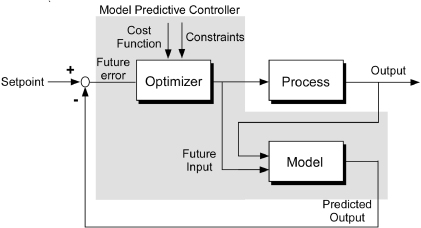
\includegraphics[scale=0.8]{Images/Chapter2/mpc_block_diagram.jpg}
\caption{Block diagram of the basic elements in Model Predictive Control \cite{Al-Sanad2005}.}
\label{fig:mpc_diagram}
\end{figure}

MPC controllers have some advantages compared to other control techniques, like the ones stated below:

\begin{itemize}

\item It can be used to control a great variety of processes, including ones that have long delay times or non-minimum phase or even unstable ones. 

\item In particular versions of MPC, it can be tuned to compensate for dead times.

\item The strategy is easily extendable to the multivariable case.

\item It can explicitly include constraints either on the control signal or the states/controlled variables.

\item It introduces feed forward in a natural way to compensate for measurable disturbances.

\end{itemize}

However, due to the characteristics of the technique, some drawbacks also arise:

\begin{itemize}

\item The main disadvantage to mention about MPC is the computing power required to solve the optimization problem in a suitable amount of time on each sampling instant, specially when the controlled systems have very fast dynamics. When the size of the problem is small, this can be solved by calculating all the possible control laws offline and then perform the look-up at runtime. However, the size of the optimization problem is also depending on the prediction horizon, which is a variable parameter considered for the tuning of the controller. This makes computational power an important aspect to consider in the implementation of MPC. Nowadays industrial computers shouldn't have problems hanlding this kind of processing, but since these are also used for several other functions, deterministic operation is important to preserve.

\item Another disadvantage of MPC is that the technique is dependant on the process model. The algorithm itself is independent of the model, but the quality of the control signal obtained through the optimization problem is strongly dependant on good predictions coming from the model. However, the integration of statistical methods of learning in recent works \cite{Bouffard2012} has been proven to solve this problem, without further modeling work.

\end{itemize}

\subsection{Model}%----------------------------------------Model--------------------------------------------------------------------------

Being of such importance to the performance of MPC controllers, the process model should be precise enough to capture all the important dynamics but simple enough to keep the optimization problem at a decent size, thus saving computational time when solving. Since MPC is not a unique strategy, different implementations of it may vary in the type of models used. However most implementations of MPC make use of one of these types of models: Transient Response, Transfer Function or State Space models. A brief description of each is presented in this section.

\begin{itemize}

\item \textbf{Transient Response.} Due to its simplicity, it is probably the most used kind of model in industry. To derive this kind of model, known inputs are fed to the real system or process and the outputs are measured. The most common inputs used for these experiments are impulse and step inputs, so in each corresponding case they are better known as impulse and step response models. The inputs and outputs are related by the following truncated sum of $N$ terms:

\begin{equation} \label{impulsemodel1}
y(k) = \sum_{i=1}^N h_i u(k-i) = H(z^{-1})u(k)
\end{equation}

where $H(z^{-1})$ is a polynomial of the backward shift operator, $z^{-1}$. For a model coming from such a simple experiment, the information that can be obtained is of great help to the understanding of the system: influenced variables by the input, time constants of the system and general characteristics can be determined from transient models. The fact that no previous knowledge of the system is required is an advantage for unknown processes. As a drawback, usually a lot of parameters are required as $N$ is usually a big number for these models.

\item \textbf{Transfer Function.} The transfer function model is obtained through the quotient of the Laplace transforms of the inputs and the outputs. When expressed in discrete time, these polynomials are a function of the backward shift operator, as stated below:

\begin{equation} \label{transferfunctionmodel1}
y(k) = \frac{B(z^{-1})}{A(z^{-1})}u(k)
\end{equation}

These models give a good physical insight and the resultant controller is of a low order and compact. However, to develop a good transfer function model some information of the system is required beforehand, more specifically about the order of the polynomials. Also, it is best suited for SISO systems.

\item \textbf{State Space.} The states of the system are described as a linear combination of the previous states and the inputs, and the output as a mapping of the states. The general form of state space models is as follows:

\begin{equation} \label{statespacemodel1}
\begin{cases} x(k + 1) = Ax(k) + Bu(k) \\ y(k) = Cx(k)
\end{cases}
\end{equation}

Where $A$ is the system matrix, $B$ is the input matrix and $C$ is the output matrix. The big advantage of this type of model is that it is straightforward to use for MIMO systems and the control law will always be a linear combination of the state vector. A drawback might be that the calculations could get complicated if a state observer is needed, as sometimes the state selection doesn't have any physical meaning.

\end{itemize}

For this thesis, the type of model used was the state space model representation. This selection allows an easier way to handle models of different sizes; also the recursive structure of the predictions from the model allows a more compact formulation of the quadratic problem, as developed by \cite{Ferreau2011}.


 
\subsection{Objective Function}%---------------------------Objective Function--------------------------------------------------------------

The objective function takes into account the error between reference trajectory and measured states, as well as the change in the control effort. The optimization process will give the values of the control signal $u$ that minimizes the values of this objective function. A basic form of this objective function would be the following:

\begin{equation} \label{objectivefunction1}
V(u) = \sum_{i=1}^{N_{p}}  [\hat{y}(k + i | k) - r(k + i)]^2 + \sum_{j=1}^{N_{c}} [\triangle u(k + i - 1)]^2
\end{equation}

Where the term $\hat{y}(k + i | k)$ represents the estimated output from the model calculated at time $k$ for any sample in the horizon, $r(k + i)$ is the reference trajectory desired for the process (which is usually known in applications such as robotics) and the term $\triangle u(k + i - 1)$ is the control effort. This objective function is quadratic, but it can also be linear or of a different order. Most MPC implementations use quadratic objective functions because they are independant on the sign of the optimised variable and they assure that a global minimum is reached. Some implementations of MPC use an approximation to the real reference trajectory which parameters can be tuned in order to adjust to fast tracking or smooth response.\\ 

Parameters $N_{p}$ and $N_{c}$ are the prediction and control horizon respectively. These can be set to the same number although it is not a necessary condition. The definition of these parameters define when it is of interest to consider the different errors. This allows the objective function to be flexible for systems with dead-times or non-minimum phase. Also these errors may have different relevance in the control of the system, therefore this objective function might include or not weight matrices in order to ponder differently the errors.\\

In this thesis, the objective function used is pre-defined by the optimization solver qpOASES, presented by \cite{Ferreau2011}, which is of the following form:

\begin{equation} \label{objectivefunction2}
V(u) = \frac{1}{2} \sum_{i=k_{0}}^{k_{0} + N_{p} - 1} (y_{k} - y_{ref})'Q(y_{k} - y_{ref}) + (u_{k} - u_{ref})'R(u_{k} - u_{ref}) + \frac{1}{2} (y_{k_{0} + n_{p}} - y_{ref})'P(y_{k_{0} + n_{p}} - y_{ref})
\end{equation}

In this equation, three sources of error are noticeable: output errors (or depending on the process, state errors), input errors and terminal cost errors. Each source has its respective weight matrix: Q, R and P, respectively. In this implementation, the prediction horizon and the control horizon have been merged into the same number $N_{p}$, simplifying the function.

\subsection{Constraints}%---------------------------------Constraints----------------------------------------------------------------------

Constraints are limitations in the values of the variables that are considered in the open loop optimization problem formulated in MPC. The explicit consideration of constraints is translated into an increase in computational complexity, as the solution of the problem can only be obtained through numerical methods. Usually, constraints in the inputs are due to limitations of the actuators interacting with the process, and constraints in the outputs or in the states come from safety or operational limits in the process itself or the sensors present in the system.\\

In \cite{Ferreau2011} a distinction is made between bounds and constraints, where the bounds are the limit values for the variable being optimised (the control signal $u$) and the constraints are expressions to define the limitations of the outputs and states, which are mapped through the matrix G as follows:

\begin{equation} \label{constraints1}
\underline{U} \leq u \leq \bar{U}
\end{equation}
\begin{equation} \label{constraints2}
\underline{A} \leq G\mathbf{x} \leq \bar{A} 
\end{equation}


\subsection{Optimization}%---------------------------Optimization--------------------------------------------------------------------------

There are two main type of algorithms used commonly to solve quadratic problems like the ones that arise in MPC: active set methods and interior point methods. A brief description of both will be presented here for informative purposes and finally, the method used in \cite{Ferreau2011} will be described.

\begin{itemize}

\item \textbf{Active Set Methods.} 

%In order to explain how these methods work, a definition for an \emph{active set} must be introduced. An optimization problem:
 
%\begin{equation} \label{eq:optimization1}
% \begin{aligned}
% & \underset{x}{\text{minimize}}
 %& & V(x) \\
 %& \text{subject to}
 %& & f_i(x) \leq b_i, \; 	i = 1, \ldots, m.
 %\end{aligned}
%\end{equation}

%is defined by the objective function and by the set of constraints. This set defines the \emph{feasible region}, which is the set of all $x$ that satisfy the constraints, and thus are considered in the search for the optimal solution. Given $x$ in the feasible region, a constraint $f$ is active in $x$ if $f_i(x) = 0$ and inactive if $f_i(x) > 0$. The \emph{active set} at $x$ comprises all the constraints that are active at that point \cite{Nocedal&Wright2006}. \\

The aim of an Active Set method is to find an optimal active set, which will make it possible to use equality constrained QP solving techniques (solving the KKT system). The algorithm will start making a guess of this optimal active set, and if it misses, gradient and Lagrange multipliers will be used to improve the initial guess. The final solution of the problem will lie in the proximity of the borders of the  feasible region.

\item \textbf{Interior Point Methods.} Given the following quadratic problem in the standard form:





Based on the KKT conditions one can say that if a given $x^*$ is a solution of \ref{eq:quadproblem}, there is a Lagrange multiplier vector $\lambda^*$ such that the following conditions are satisfied for $(x, \lambda) = (x^*, \lambda^*)$.

\begin{equation} \label{eq:KKTIP}
 \begin{subequations}
 \begin{aligned}
  Qx - A^{T}\lambda + g &= 0, \\
  Ax - b &\geq 0, \\ 
  (Ax - b)_{i}\lambda_{i} &= 0, && i = 1, 2, \ldots , m, \\
  \lambda &\geq 0. 
 \end{aligned}
 \end{subequations}
\end{equation}

If a new variable vector $y = Ax - b$ is introduced in the system, the conditions can be rewritten as follows.

\begin{equation} \label{eq:KKTIP2}
 \begin{subequations}
 \begin{aligned}
  Qx - A^{T}\lambda + g &= 0, \\
  Ax - y - b &= 0, \\ 
  y_{i}\lambda_{i} &= 0, && i = 1, 2, \ldots , m, \\
  (y, \lambda) &\geq 0. 
 \end{aligned}
 \end{subequations}
\end{equation}

Which are correspondent with the KKT conditions for linear programming problems \cite{ref:Nocedal&Wright2006}. If we assume that we are only working with a convex objective function and feasible region, these conditions are necessary but also sufficient to assure the existence of such pair, and therefore the solution of the system \ref{eq:KKTIP2} solves the quadratic problem.





\end{itemize}

\subsection{Horizons}

\chapter{Dynamic Modeling of a Quadrotor}
\label{Dynamic_Modeling_of_a_Quadrotor}
\setcounter{MaxMatrixCols}{20}

This chapter describes the modeling efforts made to develop a suitable representation of the system for the MPC library developed, based on the physical phenomena responsible for the quadrotor's operation. To start, the theoretical derivation of the quadrotor model is exposed. To verify the correct behavior of the derived model, a section is dedicated to the verification tests and their respective results. A global summary is included at the end of the chapter to compile and discuss the achievements made.

\begin{figure}[h!]
\centering
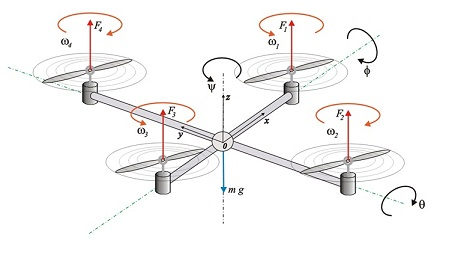
\includegraphics{Images/Chapter3/quad_dynamics.jpg}
\caption{Functioning scheme for the quadrotor dynamics. (Taken from \url{http://www.pupin.rs/RnDProfile/research-topic28.html})}
\label{fig:quadrotor_dynamics}
\end{figure}

A quadrotor has all six degrees of freedom in space and it has four actuators, which makes it an underactuated system. This means that two of the degrees of freedom must be controlled by means of regulating the other four in a proper manner. The four rotors are coupled, so the motion in the different directions is controlled by the difference in angular speed of the pairs of rotors. In Figure \ref{fig:quadrotor_dynamics}, the rotors are numbered so the pairs are defined in the directions of the axes. In order to move in the X axis, an imbalance must be made between the forces exerted by rotors 1 and 3, thus meaning a difference of angular speed in these rotors. It works the same way with the Y axis, as rotors 2 and 4 must be imbalanced as well to generate a motion in this direction. Notice that the changes in roll ($\phi$), pitch ($\theta$) angles are required to generate the motion in the X or Y directions. In order to move in the Z axis, all four rotors shall act in the same direction, therefore all four rotors must increase or decrease their angular speed. To perform a yaw ($\psi$) movement, the imbalance comes from both pairs, this is, rotors 2 and 4 rotate with a different angular speed than 1 and 3, since they rotate in opposite directions to cancel the rotating forces from the pairs and enable the quadrotor to \emph{hover} or standing still in the air.	


\section{Theoretical Derivation of the Quadrotor Model}

All known physical phenomena is used in order to obtain the theoretical model, however, the model can be as extensive as desired: in \cite{MahoneyKumarCorke2012}, the rotor aerodynamics and the concepts related to blade theory (drag and lift coefficients) are taken into consideration, however, other authors have chosen to reduce the system to use the model for control design, since these models depend on aerodynamic forces and torques, which are subjected to disturbances caused by winds and turbulence. In \cite{Hoffmann2007}, a more detailed study of the aerodynamic effects present in the quadrotor is made, but this kind of modeling is out of the scope of this report. In \cite{Bouabdallah2004} Bouabdallah et Al. state that the main physical effects present in the quadrotor system are mentioned and theoretically formulated, from which we can mention aerodynamic effects, inertial counter torques, gyroscopic effects, gravity effects and friction. However, the main effects to include for a simple model should be the gyroscopic effects of the rigid body rotation in space and the effects of the four propeller's rotation. \\

Let {$A$} and {$B$} denote two coordinate frames, where {$A$} is fixed to the ground and {$B$} is fixed to the quadrotor body in its gravity center. The relation between these two coordinate frames is defined by an homogeneous transformation given by the Euler angles, that in our case are the same angles used to determine the orientation of an airbourne vehicle: roll ($\phi$), pitch ($\theta$) and yaw ($\psi$). The transformation between {$A$} and {$B$} is defined by a rotation matrix given by the aforementioned angles and a translation vector measured from {$A$} to {$B$} as follows: 

\begin{equation} \label{eq:transformation}
\begin{pmatrix} x_A \\
				y_A \\
				z_A \end{pmatrix} = \mathbf{R_{A}^{B}}\begin{pmatrix} x_B \\
															  y_B \\
															  z_B \end{pmatrix} + \mathbf{t_{A}^{B}} 
\end{equation}

Where $\mathbf{R_{A}^{B}}$ and $\mathbf{t_{A}^{B}}$ are the rotation matrix from {$A$} to {$B$} and the translation vector from  {$A$} to {$B$}, respectively. The rotation matrix is defined as follows:

\begin{equation} \label{eq:rotationmatrix}
\mathbf{R_{A}^{B}} = \begin{bmatrix} \cos(\psi)\cos(\theta) & $\cos(\theta)\sin(\psi)$ & $ -\sin(\theta)$ \\
$\cos(\psi)\sin(\phi)\sin(\theta) - \cos(\phi)\sin(\psi)$ & $\cos(\phi)\cos(\psi) + \sin(\phi)\sin(\psi)\sin(\theta)$ & $\cos(\theta)\sin(\phi)$ \\
$\sin(\phi)\sin(\psi) + \cos(\phi)\cos(\psi)\sin(\theta)$ & $\cos(\phi)\sin(\psi)\sin(\theta) - \cos(\psi)\sin(\phi)$ & $\cos(\phi)\cos(\theta)$ \end{bmatrix}
\end{equation}

And the translation vector is simply defined as the position vector from the inertial frame ${A}$ to the body frame ${B}$. This rotation and translation together define a homogeneous transformation \textbf{T} as in equation {\ref{eq:homogeneoustransform}}.

\begin{equation} \label{eq:homogeneoustransform}
\mathbf{T_{A}^{B}} = \begin{bmatrix} \mathbf{R_{A}^{B}} & \mathbf{t_{A}^{B}} \\ 0 & 1 \end{bmatrix}
\end{equation}

If $\mathbf{v} \in A$ is the velocity of the body frame {$B$} expressed in {$A$}, $\boldsymbol{\Omega} \in B$ is the rotational velocity of the angular frame {$B$} with respect to {$A$}, expressed in {$B$}, $m$ is the quadrotor's mass and $\mathbf{I} \in \mathbb{R}^{3 \times 3}$ is the inertia matrix expressed in the body fixed frame {$B$}; a Newton's second Law of Motion force and torque balance, together with the kinematic relations between the frames lead to the following formulation:

\begin{equation} 
\begin{subequations} \label{eq:newtonformulation}
\begin{align}
	\dot{\mathbf{t}} &= \mathbf{v} \label{first}\\
	m\dot{\mathbf{v}} &= mg\hat{\mathbf{k_A}} + R\mathbf{F} \label{second}\\
	\dot{R} &= R\Omega\times\mathbf{v} \label{third}\\
	\mathbf{I}\dot{\boldsymbol{\Omega}} &= -\boldsymbol{\Omega}\times\mathbf{I}\boldsymbol{\Omega} + \boldsymbol{\tau} \label{fourth}
\end{align}
\end{subequations}
\end{equation}

When the system is expanded as scalar equations, the resultant is a 12 equation system as follows:

\begin{equation} 
\begin{subequations} \label{eq:newtonformulationexpanded}
\begin{align}
	\dot{x} &= u \label{first}\\
	\dot{y} &= v \label{second}\\
	\dot{z} &= w \label{third}\\
	\dot{u} &= \frac{1}{m}(\cos{\psi}\sin{\theta}\cos{\phi} + \sin{\psi}\sin{\phi})\mathbf{F} \label{fourth}\\
	\dot{v} &= \frac{1}{m}(\sin{\psi}\sin{\theta}\cos{\phi} - \cos{\psi}\sin{\phi})\mathbf{F} \label{fifth}\\
	\dot{w} &= \frac{1}{m}(\cos{\theta}\cos{\phi})\mathbf{F} - g\label{sixth}\\
	\dot{\phi} &= \dot{p} + q\sin{\phi}\tan{\theta} +r\cos{\phi}\tan{\theta} \label{seventh}\\
	\dot{\theta} &=  q\cos{\phi} - r\sin{\phi}\label{eighth}\\
	\dot{\psi} &= q\sin{\phi}\sec{\theta} + r\cos{\phi}\sec{\theta}\label{nineth}\\
	\dot{p} &= \frac{(I_{yy} - I_{zz})}{I_{xx}}qr - \frac{J_R\Omega}{I_{xx}}q + \frac{l}{I_{xx}}\boldsymbol{\tau_{\phi}}\label{tenth}\\
	\dot{q} &= \frac{(I_{zz} - I_{xx})}{I_{yy}}pr + \frac{J_R\Omega}{I_{yy}}p + \frac{l}{I_{yy}}\boldsymbol{\tau_{\theta}}\label{eleventh}\\
	\dot{q} &= \frac{(I_{xx} - I_{yy})}{I_{zz}}pq + \frac{1}{I_{zz}}\boldsymbol{\tau}_{\psi} \label{twelveth}\\
\end{align}
\end{subequations}
\end{equation}

Where $\mathbf{F}$ and $\boldsymbol{\tau}$ are vectors expressed in {$B$} that represent all the external forces and torques made by the aerodynamics of the rotors. These aerodynamic effects have been studied in \cite{Hoffmann2007} in depth, although this approach is unpractical in a robotics context. Nevertheless, some aerodynamics will be covered in this section to get a model that interacts at actuator level, this is, uses properties of the actuators as states. \\

For this equations system, the natural selection for the states is to choose linear and angular positions and velocities, since the derivatives of these are given in the left hand side of the set of equations 3.7. It is important to notice that these angular velocities are not equal to the derivative of the Euler angles in the mobile frame {$B$}. The derivative of the Euler angles is a discontinuous function. On the other side, the angular velocities in the mobile frame {$p, q, r$} are directly measurable through the Inertial Measurement Unit of the quadrotor, as it's actually done. From these measurements, the Euler angles are calculated \cite{Raffo2007}. Therefore we obtain a system with 12 states, as follows:

\begin{equation} \label{eq:statevector}
\mathbf{X} = \begin{bmatrix} x & y & z & u & v & w & \phi & \theta & \psi & p & q & r \end{bmatrix}
\end{equation} 

As of right now, the model takes as input the upward force coming from the combination of the thrust of the four rotors, and the three torques in space that command the orientation and angular velocities of the quadrotor frame. These quantities are difficult to measure and knowing the relationship between the rotational speeds of the actuators and these forces and torques, it is easier to think in a model where the inputs are the angular velocities of the rotors. The thrust provided by a single rotor is given by \cite{MahoneyKumarCorke2012} according to momentum theory:

\begin{equation} \label{eq:rotorthrust}
T_i = C_T\rho A_{r_{i}}r_{i}^2 \bar{\omega}^2
\end{equation}	

Where $C_T$ is the thrust coefficient for that rotor blade geometry and profile, $\rho$ is the density of air, $A_{r_{i}}$ is the rotor disk area and $\omega$ is the angular velocity. In order to perform a simpler and more practical identification, a simplified lumped-parameters model can be determined by static thrust experiments, as shown in equation \ref{eq:thrustsimple} :

\begin{equation} \label{eq:thrustsimple}
T_i = c_T \bar{\omega}^2
\end{equation}

For the case of the quadrotor, the forces and torques in space that influence the system can be decomposed in terms of the rotational speeds as follows:

\begin{equation} \label{eq:thrust_aerodynamics}
\begin{subequations}
\begin{align}
	\mathbf{F} &= c_T\bar{\omega}_1^2 + c_T\bar{\omega}_2^2 + c_T\bar{\omega}_3^2 + c_T\bar{\omega}_4^2 \label{first}\\
	\mathbf{\tau_{\phi}} &= dc_T(\bar{\omega}_2^2 - \bar{\omega}_4^2) \label{second}\\
	\mathbf{\tau_{\theta}} &= dc_T(\bar{\omega}_3^2 - \bar{\omega}_1^2) \label{third}\\
	\mathbf{\tau_{\psi}} &= c_Q((\bar{\omega}_2^2 + \bar{\omega}_4^2) - (\bar{\omega}_1^2 + \bar{\omega}_3^2)) \label{fourth}
\end{align}
\end{subequations}
\end{equation}
	
Obtaining this simplified model experimentally has the advantage that the $c_T$ coefficient includes the drag effect on the airframe that is induced due to the airflow caused by the rotor. For this model of the quadrotor, more detailed identification experiments were performed by \cite{YueSun2012}, from which the resulting parameters are taken. \\

Due to the transformation matrix, the previously presented model of the system is non-linear, and since the solver requires a linear representation, a linearization process is required. This linearization process is done using the truncated approximation to Taylor series around a certain linearization point. The performance of this model will decrease when going away from this operation point, and therefore for the purposes of MPC, the accuracy of the predictions in these cases will not be as good. There are several ways to improve this, like selecting operation points distributed around the known regions of operation of the model, so it will change the information being used depending on its current state. Another alternative is to use a variable operation point that is changed in every single iteration so the model is always in the operation point. This strategy has the downside that it implies that the system matrices will be recalculated on every iteration, consuming computational resources. The operation point used for the validation tests is presented below. This point corresponds to the quadrotor in a hover state at a determined height $z$ correspondent with the desired height of the test. \\

\begin{equation*} \label{eq:operationpoint}
\mathbf{X}^* = \begin{bmatrix} 0 & 0 & z & 0 & 0 & 0 & 0 & 0 & 0 & 0 & 0 & 0 \end{bmatrix}
\end{equation*} 

Since the objective of this thesis is not focused on modeling, a simple model with a static operation point will be used for demonstration together with the MPC software. This will have its effect on the performance of the MPC, but this effect can be reduced in some level by increasing the prediction horizon, at the cost of generating a bigger quadratic problem to solve. However, the computer running this simulation has enough processing power to handle it, but this should be highly regarded when performing this task on an onboard computer.


\section{Verification of the Model}


It is important to clarify that the following work consists only in verification, without validation. When the model is verified, its behavior is assesed to be correct, according to the described by the equations that rule the quadrotor's dynamics. However, it is not validated, in the sense that it is not proven that the model describes the behavior of the real platform. This work was not performed because the available AR Drone quadrotor takes as inputs velocity commands to an unknown control scheme programmed in the quadrotor's processing unit. Unveiling the inner control scheme in the quadrotor and bypassing it is a task that for time reasons is not performed, and therefore, the model will be simulated with the parameters identified in \cite{YueSun2012}. \\
\begin{equation} \label{eq:statevector}
\mathbf{X} = \begin{bmatrix} x & y & z & u & v & w & \phi & \theta & \psi & p & q & r \end{bmatrix}
\end{equation} 
There will be two simulations performed: one with the linearized model and one with the whole non-linear model of the platform. This is useful for the application in the MPC, where it is required to have one linear model for the platform to perform the predictions and set the quadratic problem, and the simulator for the platform, that will be represented by the full non-linear model in order to have more realistic simulations. \\

The following experiments show the outputs of the systems when a predefined set of inputs is given. These inputs are designed to obtain a specific movement pattern characteristic of the quadrotor in order to be able to analyze the outputs and assess the correctness of the outputs.These movements are the following: upwards motion along the $Z$ axis, lateral and frontal movement around the $X,Y$ axes respectively, and yaw rotation. 

\subsection{Upward motion along the X axis}

In order to generate the thrust to elevate the quadrotor, the rotors must be all operating at the same speed, above the equilibrium rotational speed (which is around 360 rad/s). 
\begin{equation} \label{eq:statevector}
\mathbf{X} = \begin{bmatrix} x & y & z & u & v & w & \phi & \theta & \psi & p & q & r \end{bmatrix}
\end{equation} 
\begin{figure}[h!]
\centering
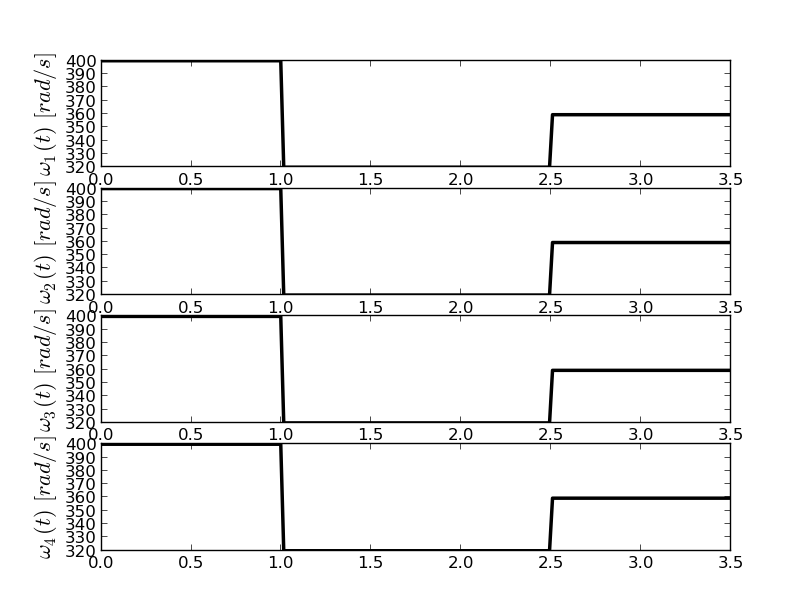
\includegraphics[scale=0.7]{Images/Chapter3/Constant_thrust_upwards/Inputs.png}
\caption{Inputs to generate an upward motion of the quadrotor.}
\label{fig:upwards_inputs}
\end{figure}

In Figure \ref{fig:upwards_inputs}, the used input signal to the model can be observed. The desired motion is an initial elevation of the quadrotor followed by a descent to some point. Therefore the signal follows this pattern. The resulting plots show the response of the simulated systems. \\

\begin{figure}[h!]
\centering
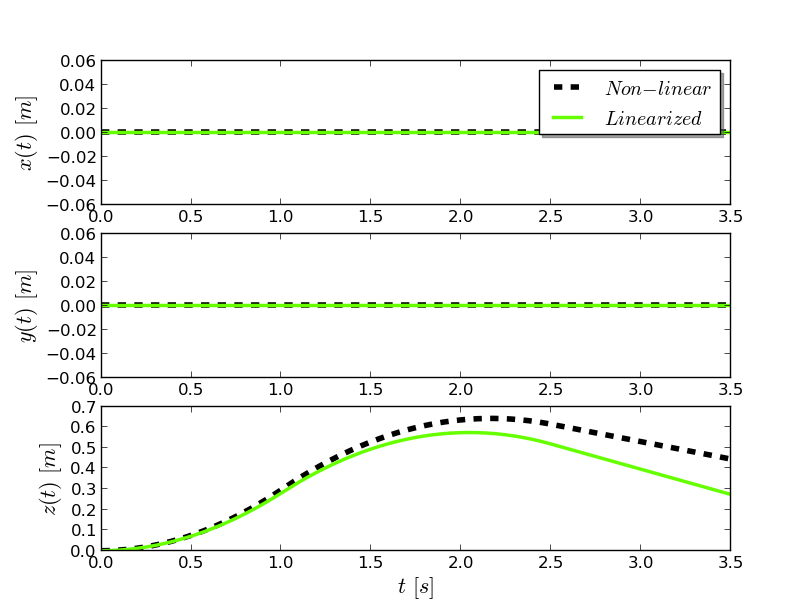
\includegraphics[scale=0.7]{Images/Chapter3/Constant_thrust_upwards/Positions.png}
\caption{Resulting positions of the simulated systems for the given inputs.}
\label{fig:upwards_positions}

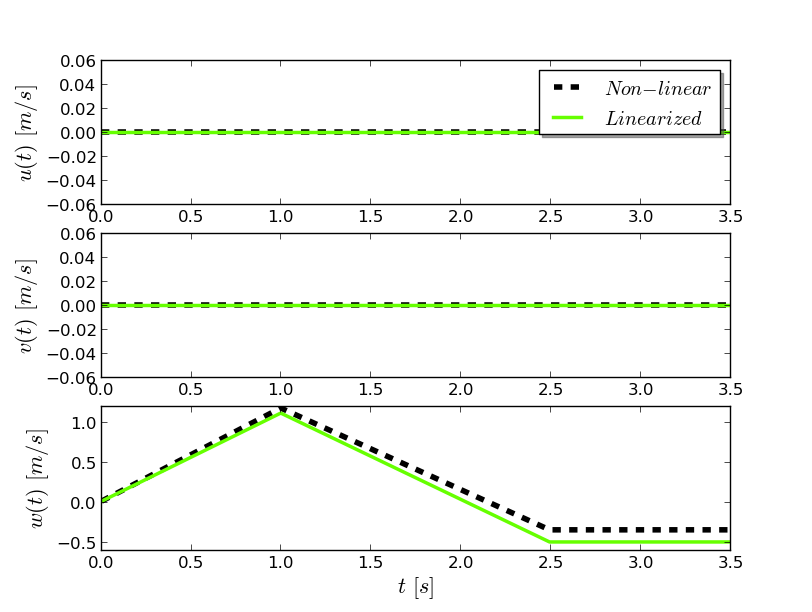
\includegraphics[scale=0.7]{Images/Chapter3/Constant_thrust_upwards/Linear_velocities.png}
\caption{Resulting velocities of the simulated systems for the given inputs.}
\label{fig:upwards_velocities}
\end{figure}

The plots for the Euler angles and the angular velocities are not shown because in this movement the angular variables are not changing. The behavior obtained is the expected in both cases, with the differences between them being caused by the linearization process. We can see that as the linear model goes further away from the linearization point the performance decreases in comparison to the non-linear model that is used as a performance reference. It is to notice that this is a simulation that doesn't take into account the ground. In Figure \ref{fig:upwards_velocities}, the velocity goes to negative values because the time that the signal goes under the equilibrium rotational speed is bigger than the time that the thrust is active, and when the equilibrium is achieved, the model keeps the negative velocity. The behavior is correct, but the absence of ground makes room for this kind of details that might confuse when verifying. \newpage

\subsection{Lateral movement along the X axis}
%\ref{eq:thrust_aerodynamics}
To move the quadrotor in the $XY$ plane, a difference in the rotor speed between the pair (1,3) must be produced as seen from equation 3.12, so the pitch torque increases and tilts the frame sideways. The design goal for the input signal was to imitate the inner controller loop in the quadrotor, since the modeling only considers the physical equipment without any control, and this system configuration is open-loop unstable. However, because of this, the signal must restore the system to its equilibrium state. The signal was obtained in an empirical way, based on the linearized and non-linear expressions that describe the system. \\

The resultant signal is a collection of pulses in opposite directions to counter each other and create the restoration effect. To have a better understanding of the effect of the signal on the model, the mapping between rotor speeds and thrust and torques acting on the quadrotor frame has been made and plotted and added below.

\begin{figure}[h!]
\centering
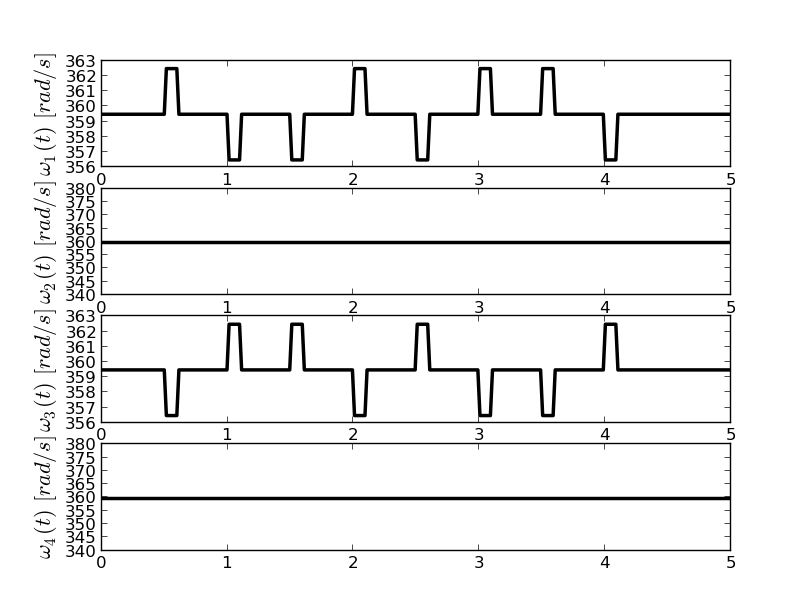
\includegraphics[scale=0.7]{Images/Chapter3/Lateral_X/Inputs.png}
\caption{Rotor speed inputs to generate a lateral movement along the X axis on the quadrotor.}
\label{fig:lateralX_inputs}
\end{figure}

\begin{figure}[H]
\centering
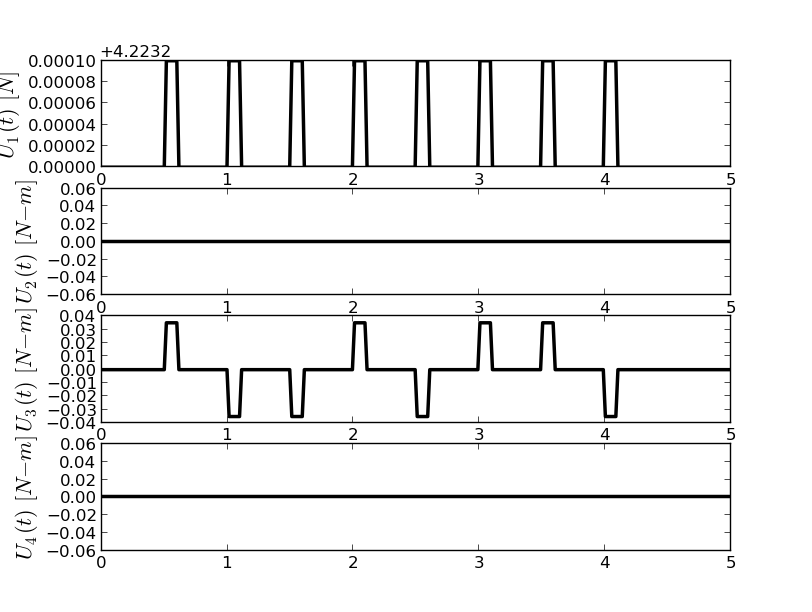
\includegraphics[scale=0.7]{Images/Chapter3/Lateral_X/Torque_inputs.png}
\caption{Rotor speed inputs from Figure \ref{fig:lateralX_inputs} mapped into forces and torques acting in the quadrotor frame.}
\label{fig:lateralX_torqueinputs}
\end{figure}


\begin{figure}[h!]
\centering
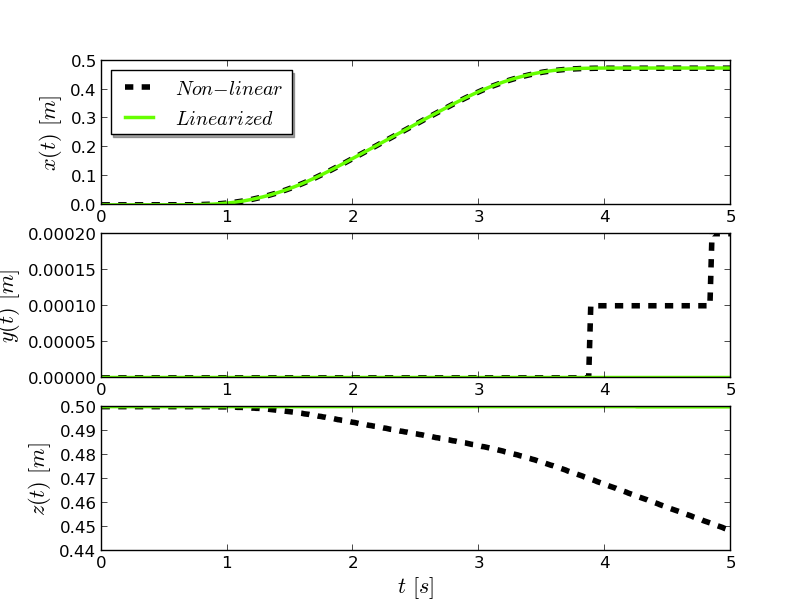
\includegraphics[scale=0.7]{Images/Chapter3/Lateral_X/Positions.png}
\caption{Resulting positions of the simulated systems for the inputs shown in Figure \ref{fig:lateralX_inputs}.}
\label{fig:LateralX_positions}

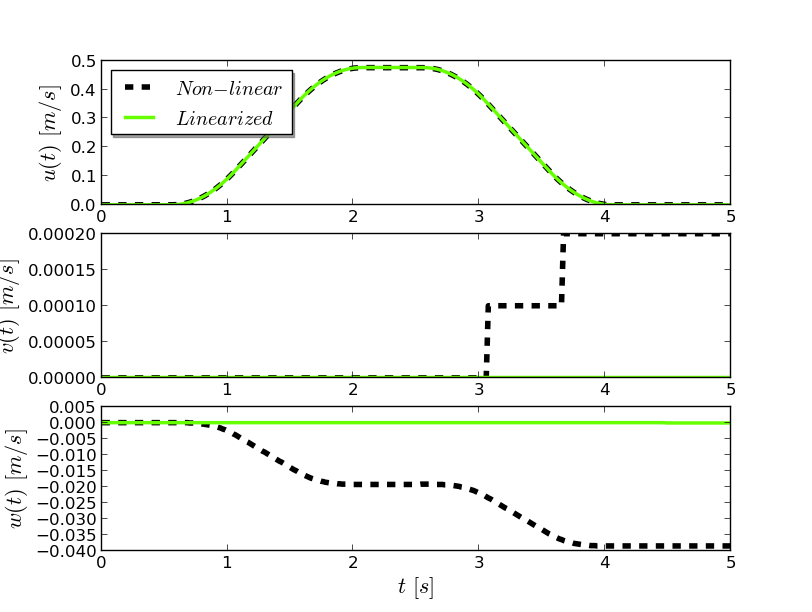
\includegraphics[scale=0.7]{Images/Chapter3/Lateral_X/Linear_velocities.png}
\caption{Resulting velocities of the simulated systems for the inputs shown in Figure \ref{fig:lateralX_inputs}.}
\label{fig:LateralX_velocities}
\end{figure}

\begin{figure}[h!]
\centering
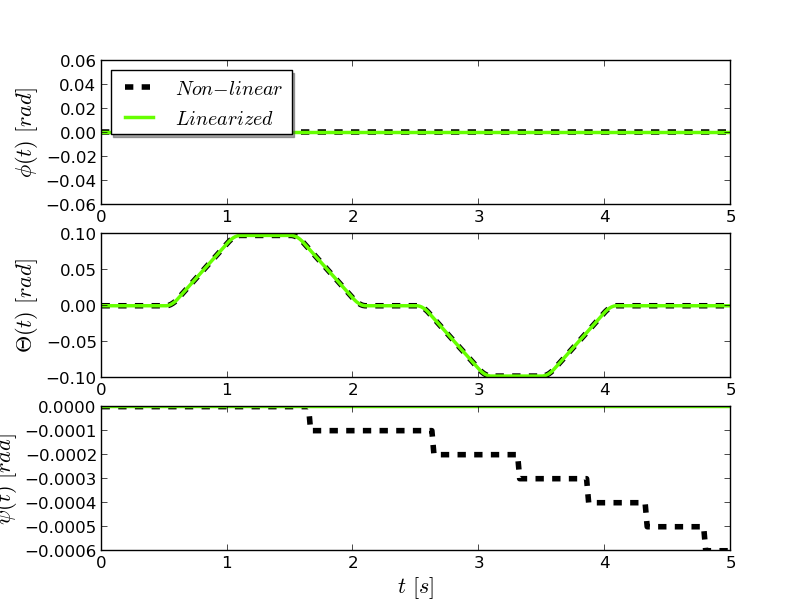
\includegraphics[scale=0.7]{Images/Chapter3/Lateral_X/Euler_Angles.png}
\caption{Resulting Euler angles of the simulated systems for the inputs shown in Figure \ref{fig:lateralX_inputs}.}
\label{fig:LateralX_Euler}

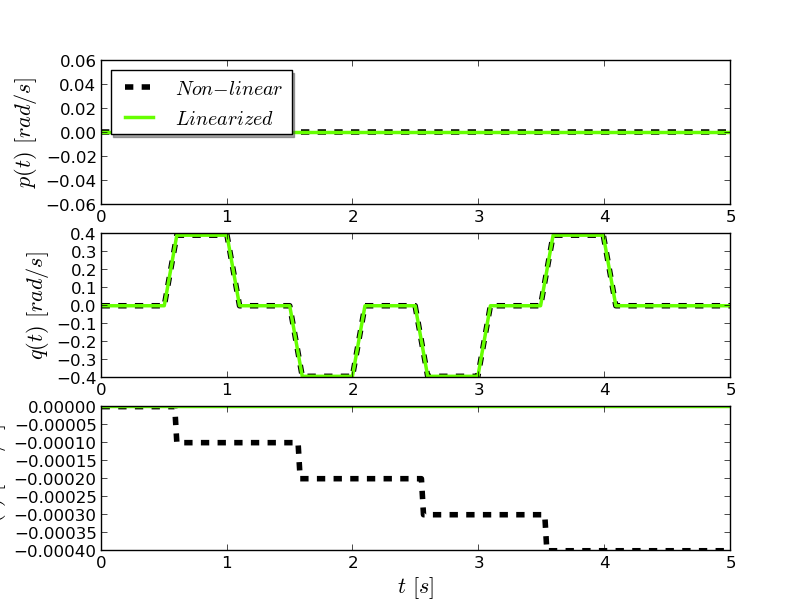
\includegraphics[scale=0.7]{Images/Chapter3/Lateral_X/Angular_velocities.png}
\caption{Resulting angular velocities of the simulated systems for the inputs shown in Figure \ref{fig:lateralX_inputs}.}
\label{fig:LateralX_angvelocities}
\end{figure}

In this simulation the quadrotor is starting from a determined height of $0.5$ meters. The resulting behavior of the model is quite satisfactory for this particular control signal. The difference between the linearized and the non-linear model is barely noticeable because the main non-linearities are introduced by the roll and pitch angles, which are kept in a very small range. Therefore, one could consider that $\cos{(\alpha)} \approx 1$ and $\sin{(\alpha)} \approx 0$. The torque inputs seen in Figure \ref{fig:lateralX_torqueinputs} are the ones calculated without the linearization process. Therefore, when a difference between a pair of rotors is stablished, there is also a slight change in the thrust, because the difference is squared. However, this difference is too small to influence the platform. This is not noticeable in the linearized output torque inputs. Another observation to highlight is that any movement of the quadrotor in any direction of the $XY$ plane will decrease a little bit the $Z$ coordinate because the thrust is redistributed for lateral movement. \newpage

\subsection{Lateral movement along the Y axis}entrenamiento en ayunas

The same input signals designed for the previous test are used in this case, only that they are applied in the (2,4) pair of rotors to switch axes.

\begin{figure}[H]
\centering
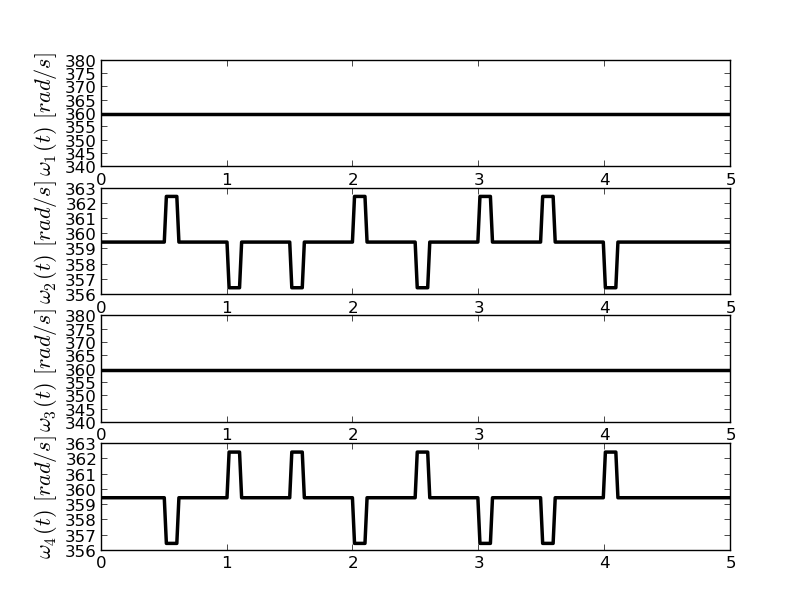
\includegraphics[scale=0.7]{Images/Chapter3/Lateral_Y/Inputs.png}
\caption{Rotor speed inputs to generate a lateral movement along the Y axis on the quadrotor.}
\label{fig:lateralY_inputs}
\end{figure}

\begin{figure}[H]
\centering
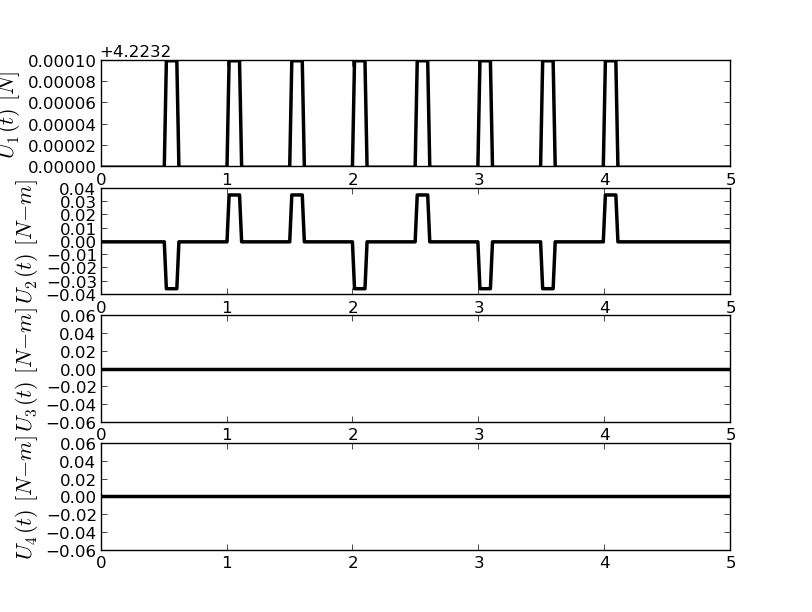
\includegraphics[scale=0.7]{Images/Chapter3/Lateral_Y/Torque_inputs.png}
\caption{Rotor speed inputs from Figure \ref{fig:lateralY_inputs} mapped into forces and torques acting in the quadrotor frame.}
\label{fig:lateralY_torqueinputs}
\end{figure}


\begin{figure}[h!]
\centering
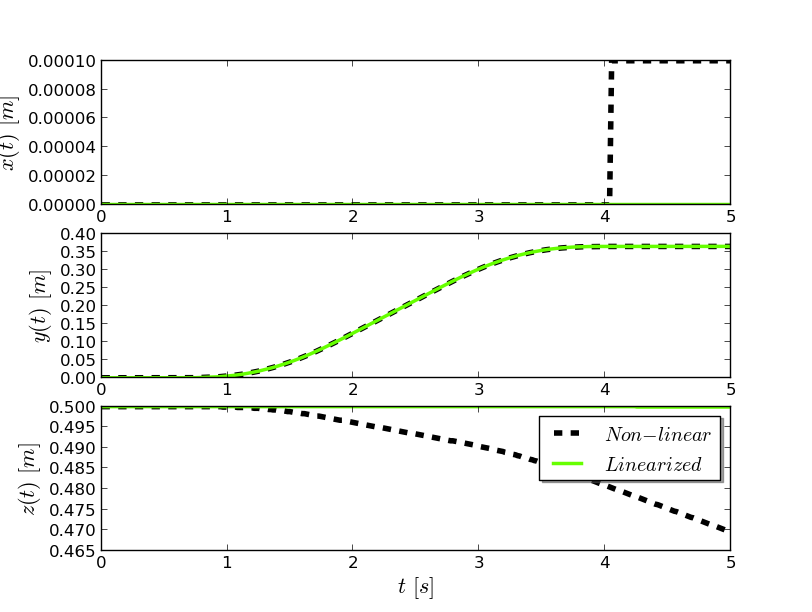
\includegraphics[scale=0.7]{Images/Chapter3/Lateral_Y/Positions.png}
\caption{Resulting positions of the simulated systems for the inputs shown in Figure \ref{fig:lateralY_inputs}.}
\label{fig:LateralY_positions}

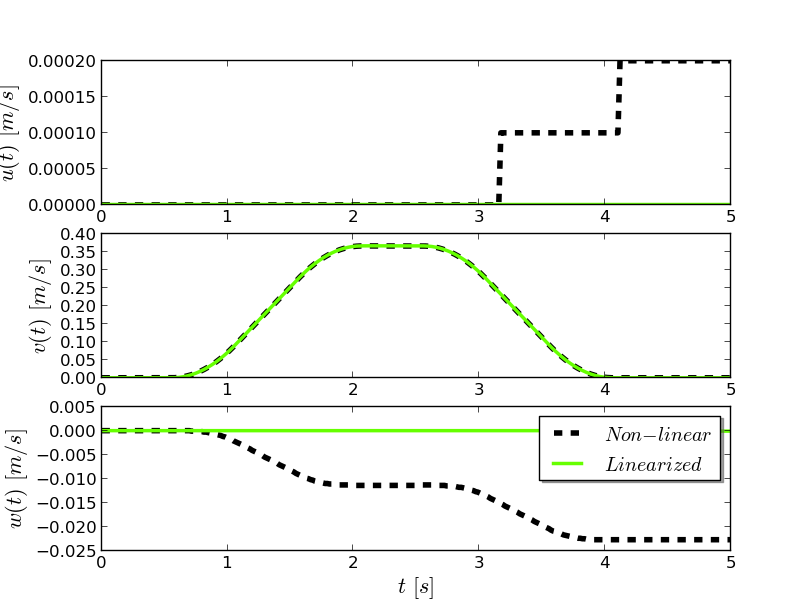
\includegraphics[scale=0.7]{Images/Chapter3/Lateral_Y/Linear_velocities.png}
\caption{Resulting velocities of the simulated systems for the inputs shown in Figure \ref{fig:lateralY_inputs}.}
\label{fig:LateralY_velocities}
\end{figure}

\begin{figure}[h!]
\centering
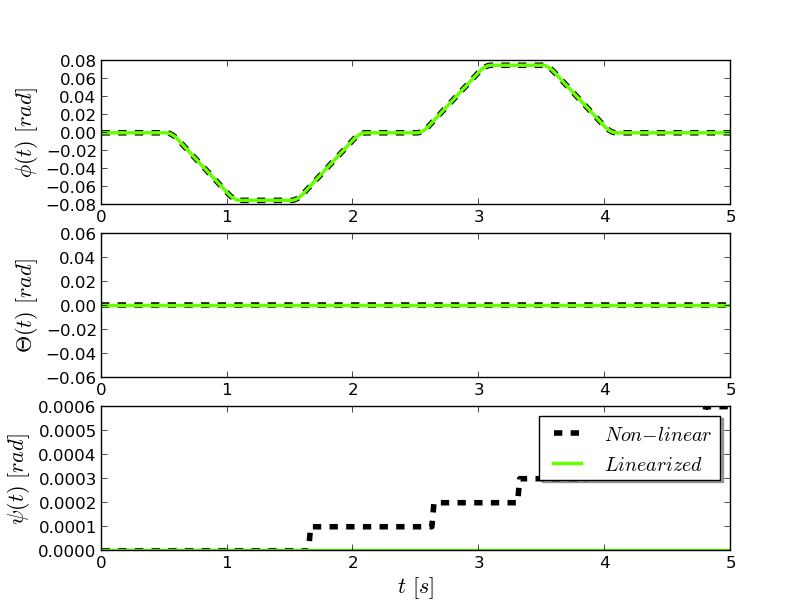
\includegraphics[scale=0.7]{Images/Chapter3/Lateral_Y/Euler_Angles.png}
\caption{Resulting Euler angles of the simulated systems for the inputs shown in Figure \ref{fig:lateralY_inputs}.}
\label{fig:LateralY_Euler}

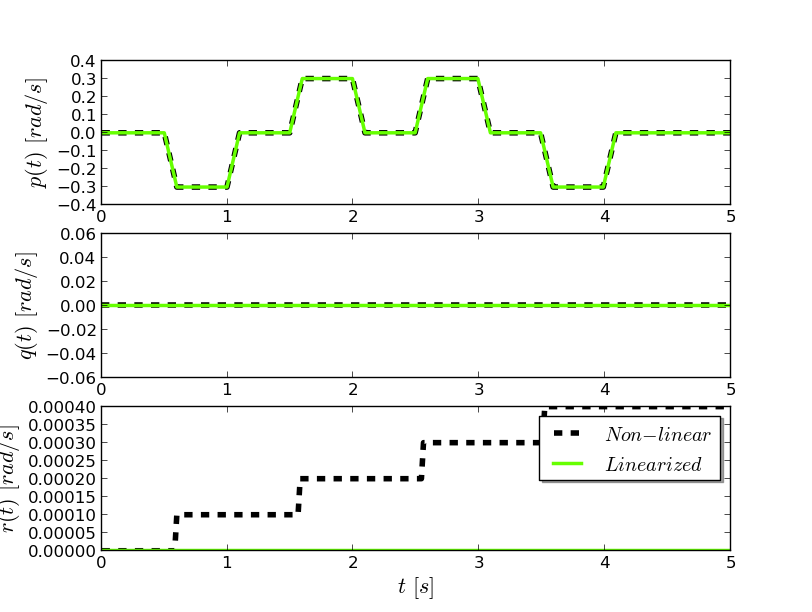
\includegraphics[scale=0.7]{Images/Chapter3/Lateral_Y/Angular_velocities.png}
\caption{Resulting angular velocities of the simulated systems for the inputs shown in Figure \ref{fig:lateralY_inputs}.}
\label{fig:LateralY_angvelocities}
\end{figure}

The resulting outputs have the same properties as the ones observed for the movement along the $X$ axis: a descent in the $Z$ coordinate caused by the coupling of the thrust force and very similar behavior between the linearized and non-linear model. In Figure \ref{fig:LateralY_positions} one can notice that the total displacement in the $Y$ axis is a little bit less in this direction, because this direction is sideways and the protective hull of the quadrotor has a bigger cross section area along this axis. 

\newpage
\section{Summary}

In this chapter a linear model of the quadrotor has been derived to integrate with the MPC software solution. This model is derived from the theoretical description of the physical phenomena responsible for the movement of the quadrotor. The quadrotor being modelled, Parrot's AR-Drone, has an inner control loop that includes the user. This is not taken in consideration in the derivation of this model. The model takes the angular speeds of the rotors as inputs and provides the quadrotor's position and yaw angle as outputs. The selection of the outputs correspond to the states being controlled, as it will be addressed later in the report. The model is linear due to a linearization process based on Taylor's series approximation, centered around a single operation point. The resulting model behaves good for small variations from this operation point. The input signals designed for the verification tests take into account that the model is open-loop unstable, so a restoring effect was required in order to obtain results that are easier and more intuitive to analyze. 


\chapter{Software Architecture and Implementation}
\label{chap:Software_Architecture_and_Implementation}

\section{Robot Operative System (ROS)}

In robotics, the amount of code required to get functional robots is quite big, since the coding goes from a driver level of the components to more higher level AI algorithms and routines. Usually, it is difficult to write code that can be adapted to several platforms or robots, and the persons in charge of this may have different choices of languages, depending on the expertise. These reasons make the integration of the different applications required to get the robot up and running a challenging work.\\

ROS is a response to these necessities, and the result is an meta-operative system designed to build a framework that provides an abstract communication layer between robotic applications in order to minimize integration efforts and reuse code. This will allow to use the same program with different platforms, accross different languages and different levels of the software, simplifying a lot the work required to develop an experimental set and making it possible to expand easily the experiments. ROS can also run in a distributed way, so that different processes can run in different computers accross a Local Area Network (LAN) \cite{QuigleyetAl2009}.\\

The ROS architecture is built in a peer-to-peer topology, where a number of processes can be running in a single host or in several hosts and communicate to each other. The coordination of the communication tasks is done by a \emph{master} process that can run in any computer in the network. The ability to run several nodes in different languages is achieved by a language-neutral interface definition language (IDL), that specifies each field of the message for the code generators and compilers of each language to generate an implementation native to the correspondent language. 

\subsection{Nomenclature}

ROS functionality can be distributed in the following elements:

\begin{itemize}

\item \textbf{Nodes} A node is any individual process in the system that performs a computational task. Nodes can be organized in a nested way, so a node can consist of several smaller nodes with distributed functionality. ROS can create a visual interface to see the organization of the currently running nodes with simple commands in the terminal.

\item \textbf{Messages} A message is the way that ROS nodes communicate between each other. It is a strictly typed data structure defined as a short text file for the compiler to interpret. A message can have primitive type like integers, doubles and floats; as well as other previously defined messages in a nested fashion.

\item \textbf{Topics} A node sends a message through topics. A topic is the channel that ROS provides to send and receive messages. A topic is defined by a string, such as "\emph{navigation}". When a node sends a message, it is said that the node has "\emph{published}" a message to a certain topic, and when it receives a message it does it by "\emph{subscribing}" to a certain topic.

\item \textbf{Services} In case of requiring syncronous communication between nodes, ROS offers services. A service consists of three elements: a string that defines the name and two strictly typed messages, one for the request and one for the response. Unlike topics, only one node can advertise a particular service with a unique name. 

\item \textbf{Parameter Server} This is a very 

\end{itemize}

\section{Library overview}

A quick description of the library can be made from Figure \ref{fig:inheritance_class_diagram} and Figure \ref{fig:implementation_class_diagram}. In Figure \ref{fig:inheritance_class_diagram}, the inheritance relationship between the interface classes and each particular instance of those classes can be seen directly here, without any functional relationship being displayed. The base classes are implemented with pure virtual functions or as interfaces; this is, they only exist through instances that inherit their methods and attributes. The interface classes cannot exist by themselves. The methods and attributes implemented in each particular application are the same, but particular implementation is defined in the derived objects.\\

The functional relation between the classes is displayed in Figure \ref{fig:implementation_class_diagram}. A particular instance of the ModelPredictiveControl interface class is responsible of solving the MPC problem, which unifies the functionality of the Model, Optimizer and Simulator (if any simulator is to be used; if not, the information is shared to the platform via ROS topic) classes.

\begin{figure}[h!]
\centering
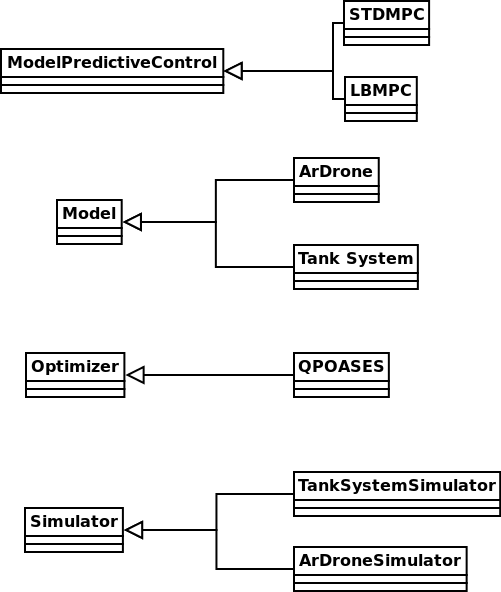
\includegraphics[scale=0.5]{Images/Chapter4/Class_Diagram.png}
\caption{Inheritance relationship between the interface and the implementation classes.}
\label{fig:inheritance_class_diagram}
\end{figure}

\begin{figure}[h!]
\centering
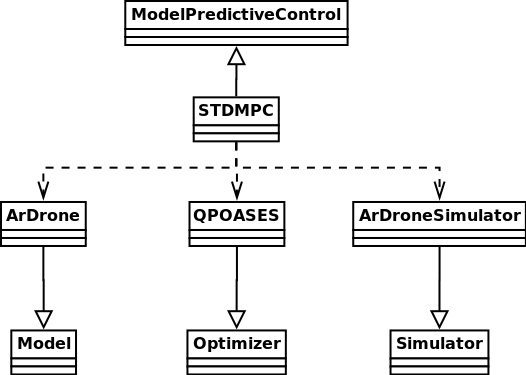
\includegraphics[scale=0.5]{Images/Chapter4/Class_diagram_implementation.png}
\caption{Implementation example of the class hierarchy for the ArDrone case.}
\label{fig:implementation_class_diagram}
\end{figure}

The main requirements for this library at the moment of its design were the following:

\begin{itemize}

\item \textbf{Expandability.} This software is thinked of so that users would know how to adapt the software easily to their specific applications with a small amount of modifications of the base program. The aim of the group is to be able to develop more functionality based on the foundational blocks of code that are created in this version. Since there are a lot of variants of the MPC algorithm, the goal is to be able to provide this options for the end user. 

\item \textbf{Modularity.} The software is designed to work with different quadratic programming solvers, different models and different simulators, just by creating derived classes from the bases that are provided. In this way, the possible combination of solvers, platforms and simulators is increased allowing for result verification and/or adapting the possible combinations to obtain the best performance for a particular application. This is also useful in order to allow to reuse code, since once a derived class for an application is completed it is ready to use in any other application available, which is why this feature is closely related to the previously mentioned expandability.

\end{itemize}

\section{Interface classes}

In this section is described in detail how each class works and integrates with each other and how they are built to achieve this goal. 

\subsection{Model}

The Model base class is used to provide the information of the dynamics of the desired model to the MPC solver. The model is provided as a linear state space model, as follows:

\begin{equation} \label{eq:model_representation}
\begin{cases}
\dot{\mathbf{x}} &= A\mathbf{x} + B\mathbf{u} \\
\mathbf{y} &= C\mathbf{x} + D\mathbf{u}
\end{cases}
\end{equation} 

So far, the only quadratic program solver that has been used provides support for models expressed in this form. If further development is continued, the aim is to provide support for the types of models that are mentioned in section \ref{impulsemodel1} and \ref{transferfunctionmodel1}.\\

The functionality of this class can be summarized in three simple actions: compute, set and get. The Model class \emph{computes} the system matrices, \emph{gets} the number of states, inputs and outputs; and \emph{sets} the states and inputs of the corresponding model.The header file provides a structure to build up upon, so that the user can define in the source file the specific information from the desired process model to be used and how these functions are being implemented. 

\begin{itemize}

\item computeDynamicModel function: this function takes the address of three Eigen matrix objects of the desired size and assigns the system matrices to those addresses as global variables for further use, returning a boolean variable to indicate success or failure. The matrices can be simply defined if the elements of each are known, or they can be calculated and discretized online when the function runs. These two ways are shown in the two different systems implemented in this thesis: in the case of the tank system, the matrices are just entered in the function so they are filled when the function runs; in the ARDrone quadrotor case, the matrices are calculated around the desired linearization point and discretized everytime the functions runs. The linearization and discretization methods are defined by the user, as long as a model with the previously mentioned structure is obtained.

\item getStatesNumber function: this function takes no inputs and returns an integer with the number of states defined by the user in the source file. The states number is stored as a global variable for further use.

\item getInputsNumber function: the same functionality as the previous get function, but with the number of inputs to the model.

\item getOutputsNumber function: the same functionality as the previous get function, but with the number of outputs of the model.

\item setStates function: this function takes an array of doubles as input and returns a boolean variable indicating success or failure at termination of the routine. The function assigns the elements of the array to the state vector array, so it is used for updating states at the end of the control loop.

\item setInputs function: this function has the same functionality as the previous set function, but with the inputs to the model.

\end{itemize}

As seen in Figure \ref{fig:implementation_class_diagram}, the Model interface class is one of the three classes that must be instantiated to be provided to an instance of the ModelPredictiveControl class to solve the MPC problem. The benefit of using an interface class is that any particular derived object can be instantiated as a pointer to the base class. This allows an easier integration between objects.

\subsection{Optimizer}

This interface class is designed to provide a way to integrate the selected quadratic programming solver to the MPC framework. Due to the variability of solvers and options available in each, this class was kept as simple as possible, to make it easier to adapt the functionality of the quadratic programming softwares and their individual options. The idea is to be able to adapt several solvers that use different methods to solve the quadratic problem depending on the structure of the problem and the particular application. \\

The integration of any solver is thinked of as a \emph{wrapper} or a frame to build upon the original functionality of the solver. The approach is to try to solve the quadratic problem including methods as simple and intuitive as possible in the class, so the details of the use of the specific solver are not required by the end user. To achieve that goal, the methods implemented were the following:

\begin{itemize}

\item init function: this function reads all the parameters required for the initialization and setting of the variables of the solver from ROS' parameter server. This function should be overloaded for each solver in particular.

\item computeOpt function: in this function the quadratic problem is solved. Several solvers require a "\emph{cold}" start run to get better approximations and improve the speed of the calculation, as is the case with qpOASES. In this particular case, it means that there are two different functions, one for the "\emph{cold}" start and one for the "\emph{hot}" start. The function recognizes this difference and launches the appropiate methods in each case. The results are stored in a protected global variable for the class. The exceptions thrown by the solver are also made easier to read and interpret for the end user, through messages that are visible in the terminal window.

\item getOptimalSolution function: this function is made to be used outside of the scope of the optimizer class instance, to be able to obtain the optimal solution, since they are protected inside the class.

\item getConstraintNumber function: this function is made to be used outside the scope of the optimizer class instance, to provide the number of constraints wherever needed.

\item getVariableNumber function: this function is made to be used outside the scope of the optimizer class instance, to provide the number of variables involved in the quadratic problem wherever needed.

\end{itemize}  

The methods of this class can be extended in the case that other software need more specific functionality. These are the functions that work with the chosen solver for this thesis, but there is a great interest of expansion in this direction to allow the user to decide which optimization algorithm suits best the application.

\subsection{Simulator}

This class is a frame for methods to simulate numerically a determined system. It works as a black-box: given some inputs and a sampling time, it delivers outputs. Since the idea is to replicate numerically as accurately as possible the behavior of the real system, the equations used in the simulator are the ones that provide the closest results to the outputs of the real system. Thus, in the quadrotor case, the equations being used to simulate are the ones from the non linear system. The functionality of this class is quite small, and it is all detailed in one single function:

\begin{itemize}

\item simulatePlant function: as described before, this function comprehends the whole functionality of the class. It takes as inputs arrays of double representing the current states, the control inputs and the sampling time; and it delivers as outputs the array of states for the next iteration. 

\end{itemize}

\subsection{ModelPredictiveControl}

This is the main class that unifies all the functionality of the previous ones to actually solve the quadratic problem posed by each MPC iteration. In the end, the methods from this class are the main methods to be used by the end user in the MPC implementation. This class also allows developers to work in their own variety of MPC, as they are a lot of varieties existing and also being developed. For example, there is currently ongoing work on developing a class to implement Learning Based Model Predictive Control, in which statistical learning algorithms are used to "learn" the non linearities and imperfections of the model and continue updating it as time goes by, thus allowing to reduce the initial modeling effort to obtain a model that is as accurate as possible. \\

All of these classes would have to adapt their main functionality to the following three methods to keep the ease of use of the library. Any additional functionality should be added in that particular class.

\begin{itemize}


\item resetMPC function: this function takes a pointer to an object of the Model, Optimizer and Simulator classes and sets the into the ModelPredictiveControl object, therefore providing the class with all the information and methods from these. Here is where the benefits of using interface classes comes into play: because of this, the pointers to the aforementioned objects can be instantiated as interface classes despite what object it is, as long as they are derived from them. This makes the implementation in the main function easily interchangeable between systems, solvers and simulators as longs as they are provided.

\item initMPC function: in this function all the parameters required to define the problem are read and all the initial calculations are performed. The parameters are read from ROS's parameter server, which can be modified without compiling afterwards using configuration files written in YAML format \cite{ClarkEvans2004}. This allows quick modifications without the time consuming compilation process.

\item updateMPC function: in this function is where the actual MPC problem is solved. The function takes the current state of the system and the desired reference for the system as inputs, and uses all the previously computed variables and parameters required to assemble the quadratic problem, then it summons the functionality from the optimizer class in order to solve the problem and provide a solution.   

\end{itemize}

\section{The Parameter Server}



\chapter{Results and Discussion}
\label{chap:Results_and_Discussion}

This chapter will be divided in three parts: in the first one, the settings and parameters to perform the tests will be presented, together with the achieved results. In the second part, an analysis of these results will be developed and the third part will be a final summary.

\section{Settings and Parameters}

Since the quadrotor has only four actuators to move in six degrees of freedom, it is an underactuated system. Hence, there will be only four variables that will be controllable. The choice made was to control the $x, y, z$ positions and the orientation around the $z$ axis ($\psi$). It is important to mention that the MPC is not sending directly the input signals going to the motors. The reason for this is that the model that is being used to perform the calculations is a linearized model, therefore the state variables represent deviations around an operation point. The MPC is instead controlling these linearized state variables and sending that to modify the initial operation point. The operation point being used is calculated by simple force balance in the hover condition, to obtain the required angular speed of the rotors to keep the quadrotor static in the air, which is approximately $360$ radians per second. That way, the control signal vector going to the quadrotor simulator is built as follows:

\begin{equation*}
\mathbf{u} = \underbrace{\mathbf{\bar{u}}}_\textrm{operation point} + \underbrace{\Delta \mathbf{u}}_\textrm{controlled by MPC}
\end{equation*}

In order to adjust to this, the constraints in the input were also modified, through a displacement of the operation range for this variation of the angular speed. The original operation range is taken from the experiments realized by Sun \cite{YueSun2012}, which is $130 \leq \omega_{i} \leq 500$, in radians per second. In order to be congruent with that range, the variation of the angular speed is limited between $-230 \leq \Delta \omega_{i} \leq 140$ around the operation point, again in radians per second.\\ 

Regarding the tuning of MPC, the parameters available to adjust are the horizons and the weight matrices in the cost function. The selection of a proper prediction horizon for any MPC application is dependant on the dynamics of the system that is being controlled.  This choice is of great influence in the size of the optimization problem to solve, and therefore in the computational power required to provide deterministic operation. If the horizon is too short, the prediction won't give information about future control signals and might create unstability in the controller \cite{Gabrielsson2012}. On the other hand, if the horizon is too long, the optimization problem to solve could be too large to solve in each time sample. In this particular case, since the model being used for prediction is a linearized version, a very long prediction in the future might mean moving too far away from the operation point, which will cause erratic predictions due to nonlinearities. \\

With the weight matrices, the procedure is also made in a trial and error fashion. A good initial guess for the quadrotor model is taken from previous implementation parameters \cite{Bouffard2012}. The simulation is performed in a computer with an Intel \textsuperscript{\textregistered} Core\texttrademark 2 Duo running at 3.0 GHz. The complete specifications for the simulation are presented in the following table.

\begin{center}
    \begin{tabular}{| l | p{7cm} |}
    \hline
    Prediction horizon & 30 samples at a frequency of 120 Hz \\ \hline
    Weight matrices & Specified in Appendix A \\ \hline
    Input constraints &  -230 \leq \Delta \omega_{i} \leq 140 [rad/s] \\ \hline
    State constraints &  -5 \leq V_x \leq 5 [m]  \newline -5 \leq V_y \leq 5 [m] \newline 0 \leq z \leq 5 [m] \\ \hline
    Processor & Intel \textsuperscript{\textregistered} Core\texttrademark 2 Duo @ 3.0 GHz
    \hline
    \end{tabular}
\end{center}

The trajectory reference used to test the MPC in the quadrotor simulator is based in simple decoupled movements in each one of the controlled directions, done one at a time. The movement consists on four stages: elevation from the floor, change in orientation (a change in the yaw angle), rotating back to the original orientation, and movements in the $X$ and $Y$ axes, in that order.\\

The results of the simulation with the mentioned parameters and settings are shown below:\\

\begin{figure}[h!]
\centering
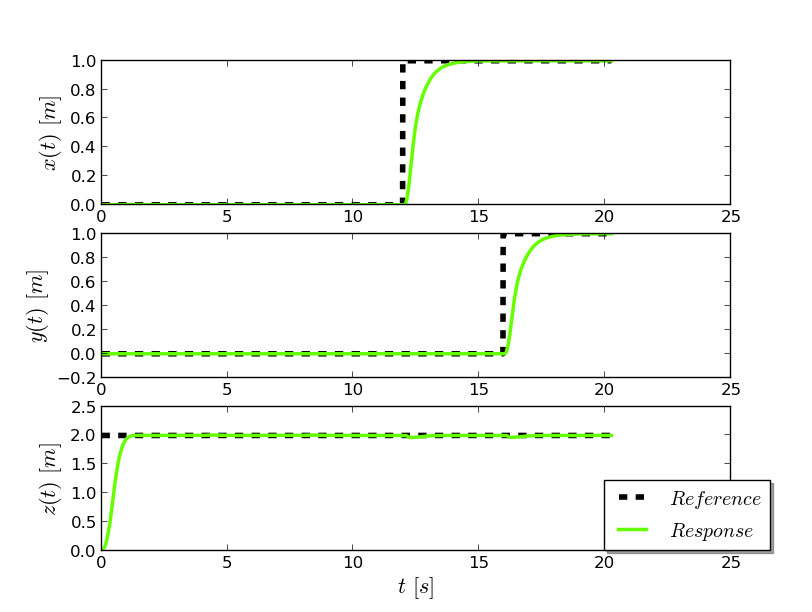
\includegraphics[scale=0.7]{Images/Chapter5/ardrone/position_control.png}
\caption{Trajectory reference and actual trajectory positions of the simulated platform.}
\label{fig:ardrone_pos}
\end{figure}

\begin{figure}[h!]
\centering
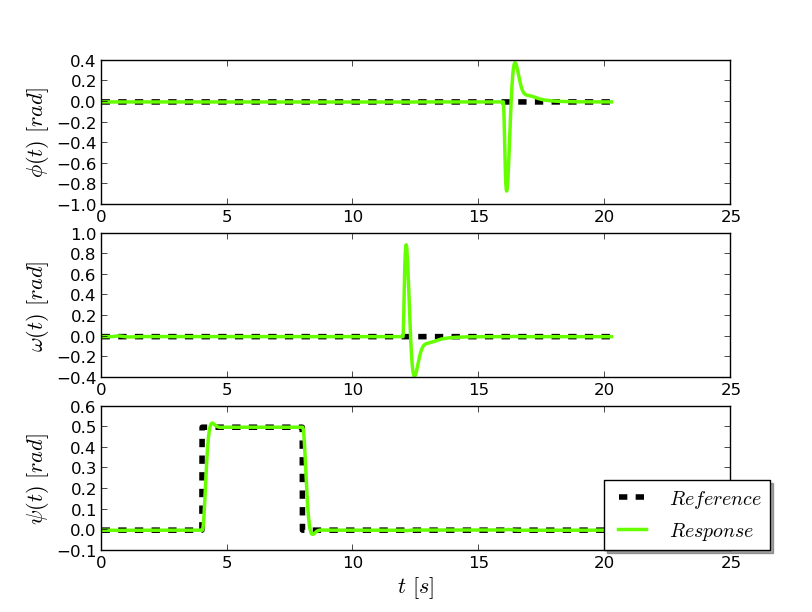
\includegraphics[scale=0.7]{Images/Chapter5/ardrone/euler_angle_control.png}
\caption{Trajectory reference and actual trajectory orientations ($\psi$) of the simulated platform.}
\label{fig:ardrone_ang}
\end{figure}

\begin{figure}[h!]
\centering
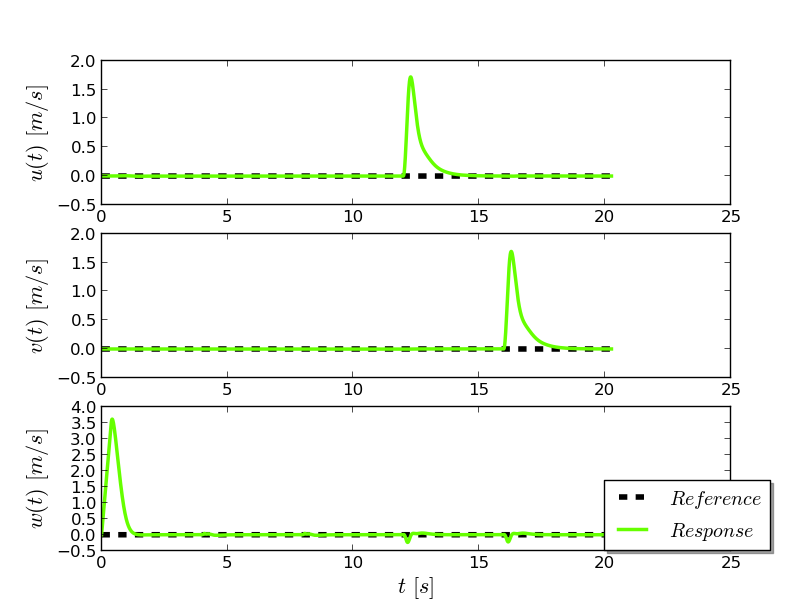
\includegraphics[scale=0.7]{Images/Chapter5/ardrone/lin_velocity_control.png}
\caption{Linear velocities of the simulated platform. }
\label{fig:ardrone_lin_vel}
\end{figure}

\begin{figure}[h!]
\centering
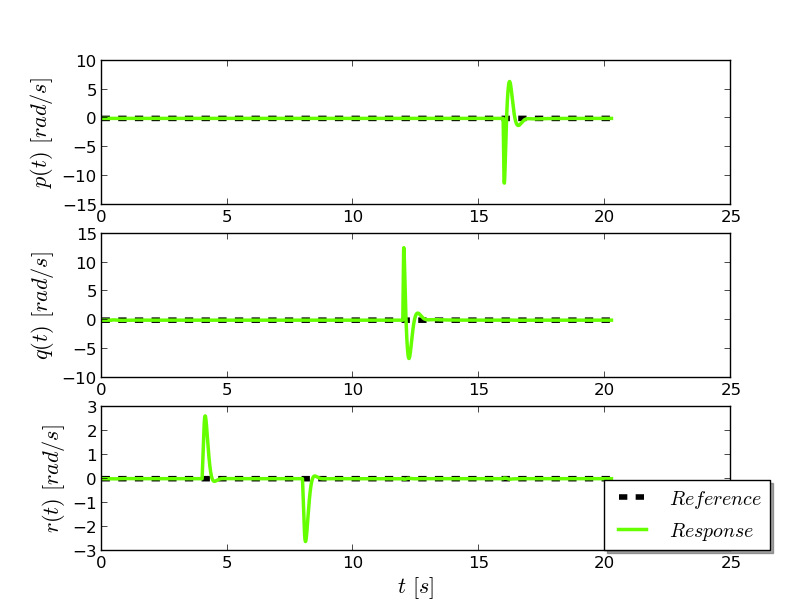
\includegraphics[scale=0.7]{Images/Chapter5/ardrone/ang_velocity_control.png}
\caption{Angular velocities of the simulated platform.}
\label{fig:ardrone_ang_vel}
\end{figure}

\begin{figure}[h!]
\centering
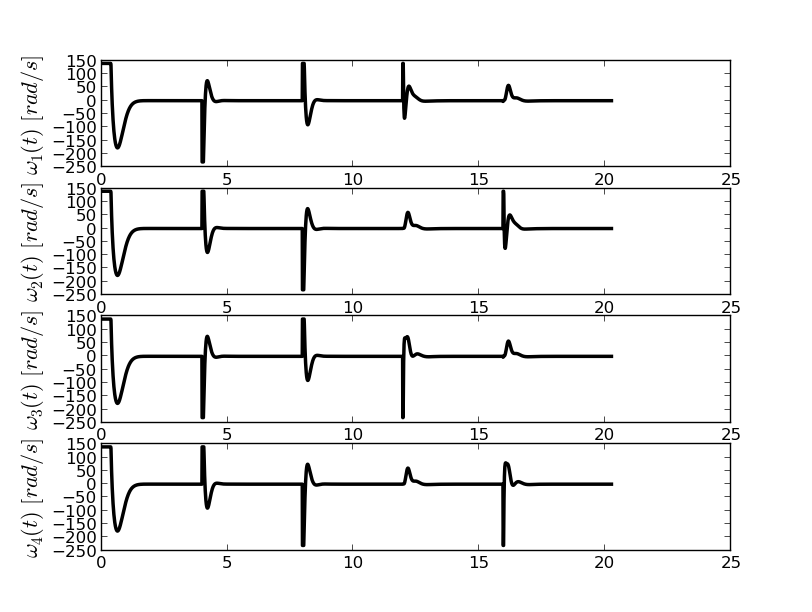
\includegraphics[scale=0.7]{Images/Chapter5/ardrone/control_signals.png}
\caption{Control signals generated by the MPC strategy.}
\label{fig:ardrone_inputs}
\end{figure}

The simulations show the performance of the MPC strategy in the simulated quadrotor. Figures \ref{fig:ardrone_pos} and \ref{fig:ardrone_ang} show the position and orientation  response of the system against step input signals on each controlled variable. The response shown presents a smooth behavior, no overshoot and a small settling time correspondant to a fast system like the quadrotor. The prediction horizon used, $N_p = 30$, has a right balance in speed to allow a fast response without overshoot.\\

The initial set of restrictions considered was bigger than the one used in the simulations shown, since there were restrictions considered on the roll and pitch angles ($\phi$ and $\theta$) taken in order to assure the stability of the quadrotor. Normally, this would be addressed by a hovering PI control loop in the original AR-Drone control architecture. However, the consideration of the constraints on these angles lead to unfeasibility in the quadratic programming problem, so  these restrictions were relaxed, and eventually dropped. The stability of the platform was addressed by strenghtening the restrictions on the velocities in the $x$ and $y$ axes, since these velocities are dependant on the roll and pitch angles. \\

The actual version of the library does not include functions to cope with unfeasibility. This must be considered in further stages of development in order to provide a better operation under the presence of more constraints. Some suggested strategies to cope with unfeasibility are referred by Camacho and Bordons \cite{CamachoBordons}: an initial strategy consists of dropping the state constraints at the initial portion of the horizon in order to make the problem feasible; another way is to create soft constraints from the hard constraints stated initially, and then adding a term in the cost function to penalize constraint violation. Feasibility is important to assure closed-loop stability. One could also use the solution of the unconstrained problem  when unfeasibility appears, but this will not guarantee stability.\\

This simulation is not performed in real-time, therefore the 




\chapter{Conclusions and Future Work}
\label{chap:Conclusions_and_Future_Work}


\bibliographystyle{plain}
\bibliography{./Bibliography/ReneDiazMPCBib.bib}
\appendix
\chapter{Appendix: MPC Parameters}
\label{chap:Appendix_A}

\section{Tank System}

\subsection{State Space matrices}

The equations of the tank:

\begin{equation}
\begin{align}
A_t\frac{dH_1}{dt} &= \beta V - A_d \sqrt{2gH_1} \\
A_t\frac{dH_2}{dt} &= A_d\sqrt{2gH_1} - A_d\sqrt{2gH_2}
\end{align}
\end{equation}

After a linearization process:

\begin{equation} \label{eq:appendix1}
\begin{bmatrix} \dot{H_1} \\ \dot{H_2} \end{bmatrix} = \begin{bmatrix} -\frac{A_d \sqrt{2g}}{2A_t \sqrt{H_{1}*}} & 0  \\ \frac{A_d \sqrt{2g}}{2A_t \sqrt{H_{1}*}} & \frac{-A_d \sqrt{2g}}{2A_t \sqrt{H_{2}*}} \end{bmatrix} \begin{bmatrix} H_1 \\ H_2 \end{bmatrix} + \begin{bmatrix} \frac{\beta}{A_t} \\ 0 \end{bmatrix} \mathbf{V}
\end{equation} 

Substituting the values of $\beta$ = 3.96, A_t = 15.52 [$cm^2$], A_d = 0.178 [$cm^2$], and discretizing with Backward Euler approximation and a sampling period of 0.01 seconds:

\begin{equation} \label{eq:appendix2}
\begin{bmatrix} \dot{H_1} \\ \dot{H_2} \end{bmatrix} = \begin{bmatrix} 0.9992 & 0  \\ -0.000803 & 1.001 \end{bmatrix} \begin{bmatrix} H_1 \\ H_2 \end{bmatrix} + \begin{bmatrix} 0.002551 \\ 0 \end{bmatrix} \mathbf{V}
\end{equation} 

\subsection{Weight matrices}

State error weight matrix:

\begin{equation*}
\mathbf{P} = \begin{bmatrix} 100.0 & 0 \\ 0 & 200.0 \end{bmatrix}
\end{equation*} 

Input Error weight matrix

\begin{equation*}
\mathbf{Q} = 0.001
\end{equation*} 

Terminal State weight matrix:

\begin{equation*}
\mathbf{R} = \begin{bmatrix} 1000.0 & 0 \\ 0 & 1000.0 \end{bmatrix}
\end{equation*} 

\section{Quadrotor}

\subsection{State Space matrices}

From the theoretical derivation made in chapter 3, and discretizing using Backward Euler approximation and a sampling period corresponding to 120 Hz:

\begin{equation*}
\mathbf{A} = \begin{bmatrix} 1 & 0 & 0 & 0.0083 & 0 & 0 & 0 & 0 & 0 & 0 & 0 & 0 \\
0 & 1 & 0 & 0 & 0.0083 & 0 & 0 & 0 & 0 & 0 & 0 & 0 \\
0 & 0 & 1 & 0 & 0 & 0.0083 & 0 & 0 & 0 & 0 & 0 & 0 \\
0 & 0 & 0 & 1 & 0 & 0 & 0 & 0.081423 & 0 & 0 & 0 & 0 \\
0 & 0 & 0 & 0 & 1 & 0 & -0.081423 & 0 & 0 & 0 & 0 & 0 \\
0 & 0 & 0 & 0 & 0 & 1 & 0 & 0 & 0 & 0 & 0 & 0 \\
0 & 0 & 0 & 0 & 0 & 0 & 1 & 0 & 0 & 0.0083 & 0 & 0 \\
0 & 0 & 0 & 0 & 0 & 0 & 0 & 1 & 0 & 0 & 0.0083 & 0 \\
0 & 0 & 0 & 0 & 0 & 0 & 0 & 0 & 1 & 0 & 0 & 0.0083 \\
0 & 0 & 0 & 0 & 0 & 0 & 0 & 0 & 0 & 1 & 0 & 0 \\
0 & 0 & 0 & 0 & 0 & 0 & 0 & 0 & 0 & 0 & 1 & 0 \\
0 & 0 & 0 & 0 & 0 & 0 & 0 & 0 & 0 & 0 & 0 & 1 \end{bmatrix}
\end{equation*}

\begin{equation*}
\mathbf{B} = \begin{bmatrix} 0 & 0 & 0 & 0 \\
0 & 0 & 0 & 0 \\
0 & 0 & 0 & 0 \\
0 & 0 & 0 & 0 \\
0 & 0 & 0 & 0 \\
1.1325e-04 & 1.1325e-04 & 1.1325e-04 & 1.1325e-04 \\
0 & 0 & 0 & 0 \\
0 & 0 & 0 & 0 \\
0 & 0 & 0 & 0 \\
0 & -8.365e-03 & 0 & 8.365e-03 \\
0.0109 & 0 & -0.0109 & 0 \\
-3.6788e-04 & 3.6788e-04 & -3.6788e-04 & 3.6788e-04 \end{bmatrix}
\end{equation*}

\subsection{Weight matrices	}

The definite matrices chosen for the simulations of the quadrotor are presented as follows:

State Error weight matrix:

\begin{equation*}
\mathbf{P} = \begin{bmatrix} 25.0 & 0 & 0 & 0 & 0 & 0 & 0 & 0 & 0 & 0 & 0 & 0 \\
0 & 25.0 & 0 & 0 & 0 & 0 & 0 & 0 & 0 & 0 & 0 & 0 \\
0 & 0 & 30.0 & 0 & 0 & 0 & 0 & 0 & 0 & 0 & 0 & 0 \\
0 & 0 & 0 & 1.0 & 0 & 0 & 0 & 0 & 0 & 0 & 0 & 0 \\
0 & 0 & 0 & 0 & 1.0 & 0 & 0 & 0 & 0 & 0 & 0 & 0 \\
0 & 0 & 0 & 0 & 0 & 1.0 & 0 & 0 & 0 & 0 & 0 & 0 \\
0 & 0 & 0 & 0 & 0 & 0 & 0.001 & 0 & 0 & 0 & 0 & 0 \\
0 & 0 & 0 & 0 & 0 & 0 & 0 & 0.001 & 0 & 0 & 0 & 0 \\
0 & 0 & 0 & 0 & 0 & 0 & 0 & 0 & 30.0 & 0 & 0 & 0 \\
0 & 0 & 0 & 0 & 0 & 0 & 0 & 0 & 0 & 0.01 & 0 & 0 \\
0 & 0 & 0 & 0 & 0 & 0 & 0 & 0 & 0 & 0 & 0.01 & 0 \\
0 & 0 & 0 & 0 & 0 & 0 & 0 & 0 & 0 & 0 & 0 & 0.01 \end{bmatrix}
\end{equation*}

Input Error weight matrix:

\begin{equation*}
\mathbf{Q} = \begin{bmatrix} 0.00001 & 0 & 0 & 0 \\
0 & 0.00001 & 0 & 0 \\
0 & 0 & 0.00001 & 0 \\
0 & 0 & 0 & 0.00001 \end{bmatrix}
\end{equation*}

Terminal State weight matrix:

\begin{equation*}
\mathbf{R} = \begin{bmatrix} 30.0 & 0 & 0 & 0 & 0 & 0 & 0 & 0 & 0 & 0 & 0 & 0 \\
0 & 30.0 & 0 & 0 & 0 & 0 & 0 & 0 & 0 & 0 & 0 & 0 \\
0 & 0 & 120.0 & 0 & 0 & 0 & 0 & 0 & 0 & 0 & 0 & 0 \\
0 & 0 & 0 & 1.0 & 0 & 0 & 0 & 0 & 0 & 0 & 0 & 0 \\
0 & 0 & 0 & 0 & 1.0 & 0 & 0 & 0 & 0 & 0 & 0 & 0 \\
0 & 0 & 0 & 0 & 0 & 1.0 & 0 & 0 & 0 & 0 & 0 & 0 \\
0 & 0 & 0 & 0 & 0 & 0 & 0.01 & 0 & 0 & 0 & 0 & 0 \\
0 & 0 & 0 & 0 & 0 & 0 & 0 & 0.01 & 0 & 0 & 0 & 0 \\
0 & 0 & 0 & 0 & 0 & 0 & 0 & 0 & 120.0 & 0 & 0 & 0 \\
0 & 0 & 0 & 0 & 0 & 0 & 0 & 0 & 0 & 0.01 & 0 & 0 \\
0 & 0 & 0 & 0 & 0 & 0 & 0 & 0 & 0 & 0 & 0.01 & 0 \\
0 & 0 & 0 & 0 & 0 & 0 & 0 & 0 & 0 & 0 & 0 & 0.01 \end{bmatrix}
\end{equation*}






\chapter{Appendix: Library Documentation}
\label{chap:Appendix_B}

\newpage
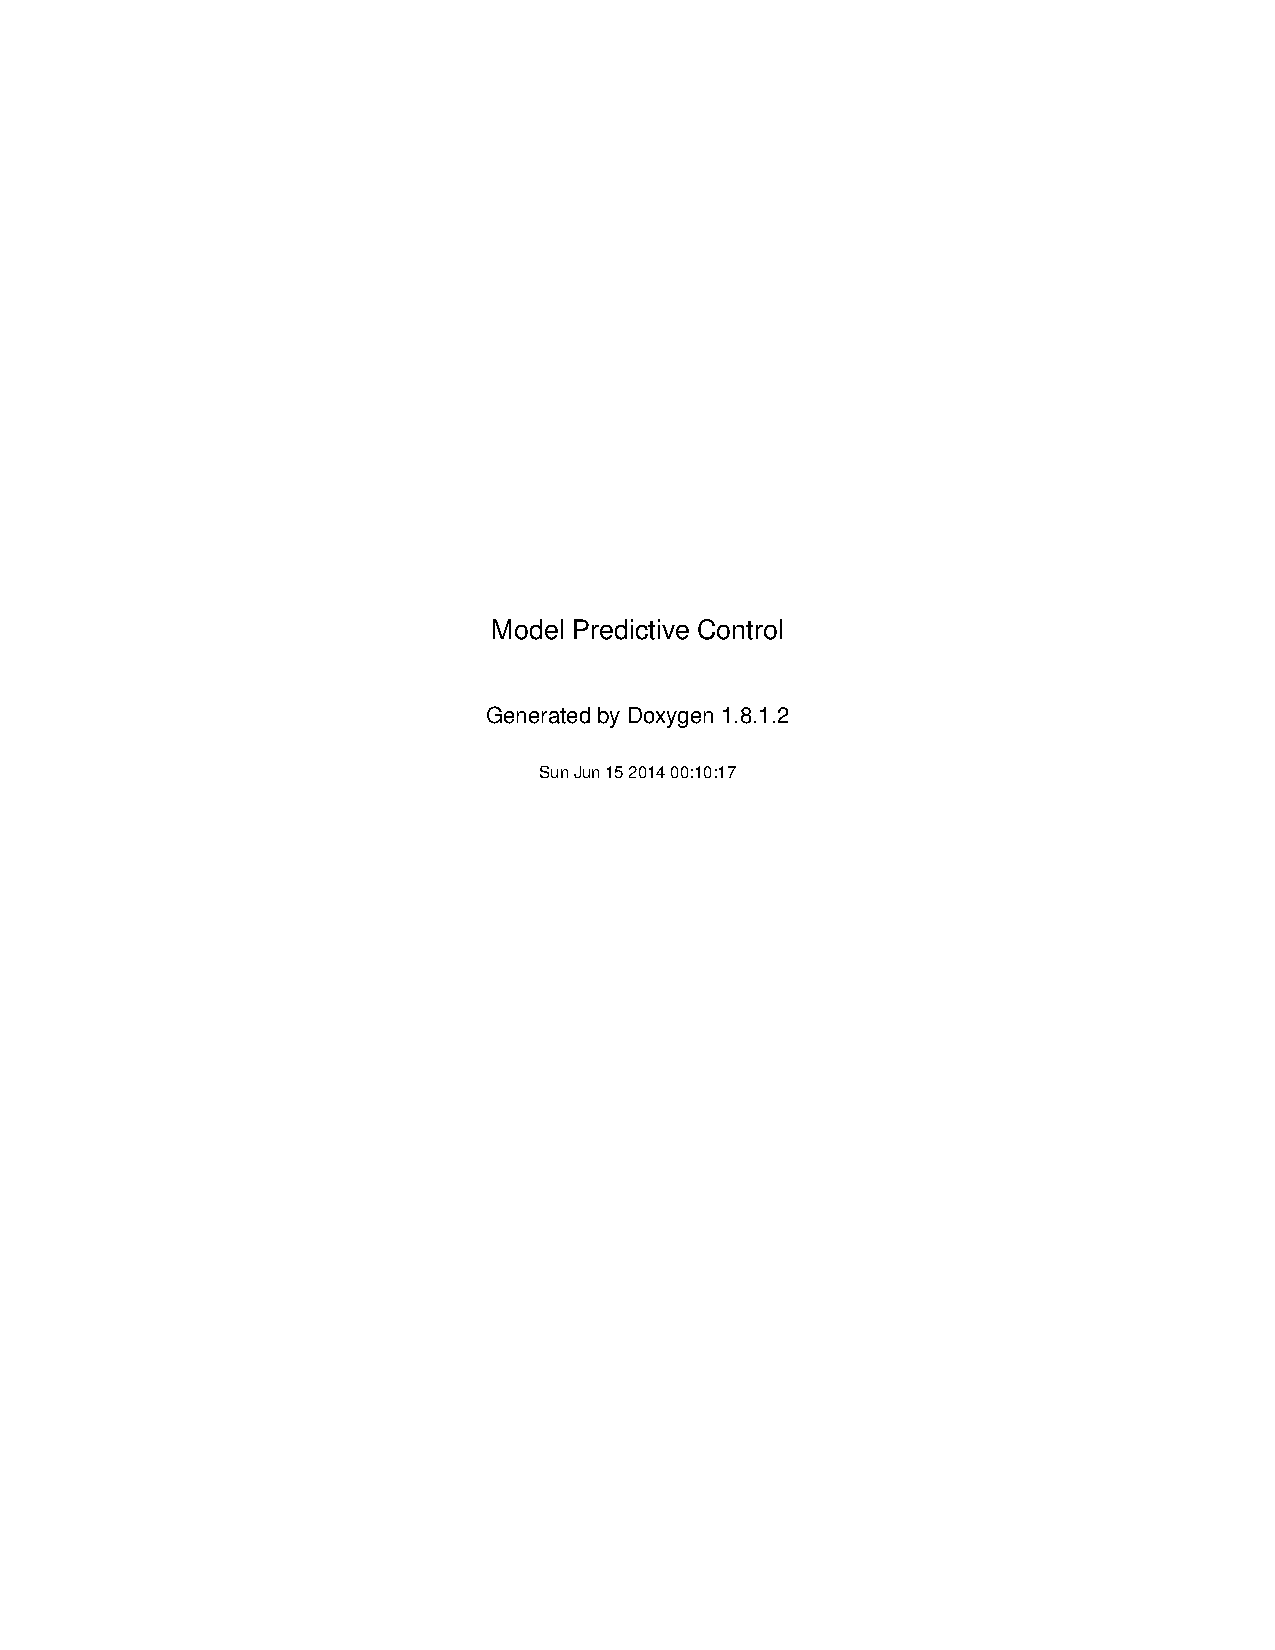
\includepdf[pages={1,19-44}]{./Appendix/refman.pdf}







\end{document}
